% ---------------------------------------------------------------------------- %
% file: disseration-coadvisors.tex
% author: Peter DeWitt
%
% LaTeX based on work by Sarah Kreidler and Peter DeWitt
% (github.com/dewittpe/ucd-dissertation-template)
%
% This is an example with Co-Advisors.  See dissertation.tex if you have a
% single advisor.
%
% ---------------------------------------------------------------------------- %

\documentclass[english,10pt]{ucdenver-dissertation}
\input{usepackages}
%%%%%%%%%%%%%%%%%%%%%%%%%%%%%%%%%%%%%%%%%%%%%%%%%%%%%%%%%%%%%%%%%%%%%%%%%%%%%%%%
% newcommands.tex

% itemize with the explaining text left justified afer the item
% Example:
%   \itembox{CNR} The Control net reduction
%   \itembox{A} Another item
% renders as
% * CNR   The Control net reduction
% * A     Another item
\newcommand{\itembox}[1]{\item {\makebox[0.80in]{#1 \hfill}}}

% Abbreviations 
\newcommand{\ie}{{\itshape i.e.}}
\newcommand{\eg}{{\itshape e.g.}}

% Bold symbols
\newcommand{\bs}[1]{\boldsymbol{#1}}

% Cardinality
\newcommand{\card}[1]{n\left(#1\right)} %{\left|#1\right|}

% Math Operators
\DeclareMathOperator*{\argmin}{arg\,min}
\DeclareMathOperator*{\argmax}{arg\,max}

% Standard Probability
\DeclareMathOperator{\E}{\mathbb{E}}
\DeclareMathOperator*{\P}{\mathbb{P}}

% Data-Consistent Inversion Framework


% Parameter Space

\DeclareMathOperator*{\param}{\lambda}
\DeclareMathOperator*{\pspace}{\Lambda}
\newcommand{\pmeas}{\mu_{\pspace}}
\newcommand{\pborel}{\mathcal{B}_{\pspace}}

\DeclareMathOperator*{\initialP}{\P_{\text{in}}}
\DeclareMathOperator*{\initial}{\pi_{\text{in}}}
\DeclareMathOperator*{\updatedP}{\P_{\text{up}}}
\DeclareMathOperator*{\updated}{\pi_{\text{up}}}

\DeclareMathOperator*{\data}{\boldsymbol{d}}
\DeclareMathOperator*{\dspace}{\mathcal{D}}
\newcommand{\dmeas}{\mu_{\dspace}}
\newcommand{\dborel}{\mathcal{B}_{\dspace}}

\DeclareMathOperator*{\q}{Q\left (\param \right )}
\DeclareMathOperator*{\M}{\mathcal{M}}

\DeclareMathOperator*{\obsP}{\P_{\text{ob}}}
\DeclareMathOperator*{\obs}{\pi_{\text{ob}}}
\DeclareMathOperator*{\predP}{\P_{\text{pr}}}
\DeclareMathOperator*{\pred}{\pi_{\text{pr}}}




%%%%%%%%%%%%%%%%%%%%%%%%%%%%%%%%%%%%%%%%%%%%%%%%%%%%%%%%%%%%%%%%%%%%%%%%%%%%%%%%

 

\usepackage{lipsum}

\widowpenalty=10000
\clubpenalty=10000
\renewcommand{\floatpagefraction}{0.7}%

% Draft and Time stamp in the header and footer.
% \usepackage{fancyhdr}
% \usepackage{datetime}
% \lhead{\color{red} DRAFT: \today; \currenttime}
% \rfoot{\color{red} DRAFT: \today; \currenttime}

% \doublespacing
\onehalfspacing

% ---------------------------------------------------------------------------- %
% FRONT MATTER i

\makeatletter
\title{Computational Advances in Data-Consistent Inversion: Measure-Theoretic Methods for Improving Predictions}
\authorLast{Pilosov}
\authorFirst{Michael}
\authorMiddle{}
\education{
B.A., State University of New York: College at Geneseo, 2010 \\
M.S., University of Colorado: Denver, 2015
}
\school{University of Colorado: Denver, College of Liberal Arts and Sciences}
\program{Applied Mathematics}
\date{2019}
\submitDate{21 Sep 2019}
\advisor{Dr.~Troy Butler}
\advisorTitle{Assistant Professor}
\committeeChair{Dr.~Stephen Billups}
\committeeMembers{
Dr.~Varis Carey \\ 
Dr.~Jan Mandel \\
Dr.~Jimmy Lee Kim 
}

% dedication - this is also optional
\dedication{To Jacob and Anna Ratman.}

% preface
\preface{
This work is concerned with presenting novel developments in the solution of stochastic inverse problems in a measure-theoretic framework which leverages push-forward and pull-back measures.
Previous work focused on transforming distributions based on the differences between push-forward and observed measures rather than the popular Bayesian approach of updating prior beliefs with likelihood functions.
The primary contributions herein revolve around extending the Data-Consistent Inversion framework to address problems that seek to identify a single ``true'' parameter from the aggregation and use of noisy data. 
Prior work was developed around problems that quantified parameter variability inherent to natural processes such as manufacturing or experimental setup, leaving no need to presume the existence of a single parameter value that explained variations in observational data.
However, many scientific problems are inherently grounded in such a belief, and so we are motivated to extend the Data-Consistent Inversion framework to address such scenarios in hopes that it can provide feasible alternatives to Bayesian Likelihood approaches.

As such, this work sits at the intersection of applied mathematics, science, and computation.
The scientific ``laboratory'' in which we perform our (simulated) experiments is the computer. 
Since computation plays such an integral part in the process of answering the aforementioned questions, a considerable amount of attention is also devoted to addressing software development. 
A novel method whose implementation is difficult to use is unlikely to see widespread adoption, so in the interest of making our work as accessible as possible, a lot of non-mathematical content is presented.
This work will demonstrate in detail how the open-source tools we developed were built and delivered to the scientific community. 
}


% acknowledgement - this is optional
\acknowledgements{ 
  Thank you to Troy Butler, whose patient guidance got me through this grueling process.
}

\usepackage{array}
\renewcommand\arraystretch{0.5}

\makeatother

% ---------------------------------------------------------------------------- %
% ---------------------------------------------------------------------------- %
% Begin Document 
\begin{document}
\section*{Outline}

\begin{description}[leftmargin=!, labelwidth=0.7in]
\item[Chapter 1] Introduction

\item[Chapter 2] Background on Data Consistent Inversion:
\begin{description}[leftmargin=!, labelwidth=0.7in]
	\item[Section 2.1] Notation, Terminology, and Assumptions
	\item[Section 2.2] Set-Based Inversion for Measures
	\item[Section 2.3] Sample-Based Inversion for Densities
	\item[Section 2.4] Software Contributions (description of your updating of BET to Python 3 that you are doing for NSF goes here along with including the newer approach with densities that you are adding to BET, discuss testing, installation, etc. at a high level)
	\item[Section 2.5] Illustrative Examples
\end{description}

\item[Chapter 3] Impact of Output Quantities on Accuracy
\begin{description}[leftmargin=!, labelwidth=0.7in]
\item[Section 3.1] Skewness and Information Content (this is a review section)
\item[Section 3.2] Skewness and Accuracy of Set-Based Inversion (this is a summary of your MS work updated for TV metric)
\item[Section 3.3] Skewness and Accuracy of Sample-Based Inversion (newer work that you were doing but hadn't written up yet, focus on linear problems and how KDEs deal with skewness on the data space)
\item[Section 3.4] Software contributions (adding the module to BET that computes the TV metric that is updated from your MS work, also discuss testing, and simple examples of usage that are disconnected from skewness, mostly high level)
\item[Section 3.5] Numerical results and analysis
\end{description}

\item[Chapter 4] Data-driven maps and Consistent Inversion
\begin{description}[leftmargin=!, labelwidth=0.7in]
\item[Section 4.1] A Generalized Stochastic Map Framework (material from the paper I am finishing up -- hopefully in the next two weeks for first draft -- goes here to set the stage)
\item[Section 4.2] Data-driven maps (also material from the paper including sensitivity analysis as the number of data points $M$ increases)
\item[Section 4.3] Software contributions (adding a module in BET to transform time series into QoI and do the data-consistent inversion)
\item[Section 4.4] Numerical Results and Analysis
\end{description}

\item[Chapter 5] Other Research from NSF project yet to be done/defined well enough to sketch out this chapter - perhaps functional assimilation discussion? Maybe no chapter 5 on this? We will see.
 
\item[Chapter 6] Summary, Conclusions and Future Research Directions

\item[Bibliography]

\end{description}

%\chapter{\uppercase{Introduction}} \label{chapter:01}

\section{Preliminaries}

\
\section{Motivations}


\section{Software Contributions}
Everything in this thesis has been incorporated into open-source software.
The novel mathematical developments that have gone into the work herein are all reflected in various modules and sub-modules as part of the BET python package.
This software suite follows a number of industry best-practices for code-coverage and continuous integration, i.e. the code is well-tested.

A significant proportion of the effort involved in the writing of this thesis revolved around learning about the art and practice of modern (open-source) software development.
As new ideas sprang up, our research group found itself coding and re-coding the same methods that had yet to be incorporated into user-friednly, computationally efficient, and properly-parallelized libraries.
Over the years, the software fell behind the state-of-the-art in research, and previous maintainers of code had moved on from their academic positions.
The author spent most of 2019 bringing the software in-line with the latest developments in Data-Consistent Inversion.

\subsection{Architecture}
Having learned a lot about software reproducibility along the way, the author made the decision to treat this thesis as a software project in its own right.
Every example, figure, table, plot will be generated by a combination of Python and Bash scripts contained inside of an public Github repository (www.github.com/mathematicalmichael/thesis).
All the requisite LaTeX dependencies are contained in {\tt apt.txt}, and a Jupyterlab environment usable by Binder (which can compile the document and run every example) is configured in the {\tt binder/} directory of the repository.

Special care will be taken to ensure that every file herein is well-documented. When appropriate, functions and classes will be used in such a way that several examples can be generated from the same file.
The parameters required can be passed as optional arguments, and bash scripts containing the exact syntax to generate each figure will be included.

For example, to visually demonstrate the implicitly-defined sets of nearest-neighbors in two-dimensional unit domain, we rely on Voronoi-cell diagrams (figures).
One python file (\bashinline{images/voronoi_unit_domain.py}) contains the methods required to draw a figure.
Some plots require labels, and others do not, and at one point we want to demonstrate the impact of random sampling on the geometry of the induced computational equivalent of a $\sa$.
To accomodate these different plots, we utilize the argument-parsing package \pythoninline{argparse}, part of the Python standard library, to enable command-line positional and optional arguments \footnote{We equip each function with default values so that the syntax \bashinline{python example.py} without any additional arguments will work, but specific examples rely on properly-passed optional arguments.}.
Thus, we would include an associate (wrapper) file with a descriptive name, such as \bashinline{images/make_voronoi_diagrams.sh} that calls the relevant python file and passes arguments (such as {\tt num} for ``number of samples''):
\bashexternal{images/make_voronoi_diagrams.sh}.

%\chapter{\uppercase{Background on Data-Consistent Inversion} \label{chapter:02}}

\section{Notation, Terminology, and Assumptions}
\subsection{Models and Parameters}
We begin by assuming that a (deterministic) model, denoted by $$\M (u, \param) = 0,$$ is specified to relate observable state variables $u$ to model inputs ({\em parameters}) denoted by the vector $\param\in\RP$.
The components $\param_\iparam$ may include parameters in either the model operator (e.g. a diffusion coefficient) or input data (e.g. the frequency of a sinusoidal source, initial, or boundary information).
We allow $\pspace$ to denote the set of all possible input parameters.
We assume $\pspace\subset\RP$ is equipped a (volume) measure, $\pmeas$ on the Borel $\sa$ $\pborel$, defining the measure space $\Pspace$.
The solution operator of the model $\M$ then defines a map taking $\param\in\pspace$ to a solution denoted $u\lam$ which is assumed to be unique.

However, in real experimental settings we are often unable to observe $u\lam$, instead having access to some finite set of observable scalar quantities.
For example, in experiments involving the diffusion of heat, we can typically only record the temperature at some small number of pre-specified points in space-time where measurement devices can be positioned.

\subsection{Quantities of Interest}
Such observable values of $u\lam$ are mathematically modeled by functionals of the solution, denoted $\qoi_\idata: u\lam \to \RR$.
The collection of such functionals into a vector defines a {\em Quantity of Interest} (QoI) map.
Since the solution to the model depends on $\param$, so do the QoI, which motivates the notation
$$\qlam := \qoi( u\lam ) \in\RD,$$
to make this dependence on model parameters explicit.
Furthermore, this convention captures a realistic limitation of an experimental setting, where we may be able to control $\param$ in order to observe $\qlam$, but lack the ability to observe $u\lam$ directly.
The outputs of the QoI map $\qlam = \data$ are what we refer to as the \emph{data}.
Similarly, the range of the QoI defines the \emph{data space} $\dspace$, i.e.
$$\dspace = \qoi(\pspace) \subset \RD$$

We let $\qspace$ denote the set of possible QoI maps for which it is possible to collect experimental data.
For example, suppose we may record only a single temperature measurement at any of ten locations in space-time.
Then $\qspace$ is defined by ten possible QoI maps.
If we can record any two such measurements, then $\qspace$ is defined by $\binom{10}{2} = 45$ possible maps.
Observe that $\qspace$ could easily be uncountable, for example if we were not limited to the spatial locations (or time) at which we could record temperature measurements.
However, for simplicity, we will only discuss problems where $\qspace$ is finite.
In the event that we need to compare maps, we adopt the notation $\dspace_{\qoi}$ to emphasize that the data space depends on the choice of QoI map $\qoi$; when the context is clear, we drop the subscript.
The only assumption on $\qoi$ that we impose throughout this work is that of piecewise-differentiability.

\subsection{Chapter Outline}
First, we discuss set-based inversion to respect the order in which these results were researched and developed, despite the reality that in more recent practice, the approach based on sampling has proven more desirable.
In the interest of clarity of exposition, we have adapted the notation of the latter approach in order to express the construction of the former.
Consequently, the references cited may require some work translating. Similarities and differences between the two approaches has heretofore avoided formal documentation, and this work serves to lay the groundwork for such a comparison. 

In this chapter, we discuss the issues that arise from the need to numerically approximate the solutions to our inverse problems but study the implications in \ref{sec:set-sec:set-error} and \ref{sec:sample-error}.
Discussion of the impact of sample size are kept to a minimum in \ref{chapter:02} in the interest of restricting the scope of \ref{chapter:03} to the implications for convergence of (consistent) solutions to \ref{eq:inverse-problem}.

%%%%%%%%%%%%%%%%%%%%%%%%%%%%%%%%%%%%%%%%%%%%%%%%%%%%%%%%%%%%%%%%%%%%%%
\pagebreak
\section{Set-Based Inversion for Measures}\label{sec:ch02-set}
% Intro
To properly summarize the Stochastic Inverse Problem (SIP) and desired solution, we define several measure/probability spaces and refer to the schematic given in Figure \ref{fig:scheme} in order to illustrate the steps and spaces required in the formulation and solution of the SIPs we consider herein.
For a more extensive review, we refer the reader to \cite{BBE11}, \cite{BES12}, and \cite{BET+14}.
Additional background and extensions of this theory are available in the PhD theses of Lindley Graham (UT Austin), Scott Walsh (CUD), Lei Yang (CSU) [TK - cite 3].

%%%%%%%%%%%%%%%%%%%%%%%%
\begin{figure}[!h]
\begin{equation}
\underbrace{
\underbrace{
\overbrace{
 \Pspace \xmapsto{\  \qoi \ } \Dspace
  \xmapsto{\ \observedP \ } \Ospace
 }^{
 \text{(S1): Stochastic Inverse Problem (SIP)}
 }
 \xmapsto{\ \qoi^{-1} \ } (\pspace, \cborel, \contourP)
 }_{
 \text{(S2): Solution to SIP Satisfying Eq. \eqref{eq:dataspace_pushforward_measure}}}
 \xmapsto{\ \set{\PP_\ell}_{\ell\in\mathcal{L}} \ } (\pspace, \pborel, \paramP)
 }
 _{
 \text{(S3): Unique Solution to SIP by Eq.~\eqref{eq:disintegration_measure} and Ansatz}
 }
\end{equation}
\caption{The first step (S1) defines (i)~the formulation of the SIP by specification of the model, (ii)~the measure spaces of parameters and (iii)~observable outputs, and (iv)~the probability measure on the latter. The second step (S2) defines a unique solution to the SIP on the space $\pspace$ equipped with the contour $\sa$ $\cborel$ using the definition of the push-forward measure. In (S3), the Disintegration Theorem and and Ansatz are applied to define a unique solution on the space of interest $(\pspace, \pborel)$ equipped with a probability measure $\paramP$.}
\label{fig:scheme}
\end{figure}


The initial measure/probability spaces involved in the formulation of the SIP are summarized in step (S1) of Fig.~\ref{fig:scheme}, starting with measure space $\Pspace$.

The assumption that $\qoi$ is at least piecewise-differentiable implies the measurability of the QoI map, so that the space $\dspace$ induced by $\qoi$ is equipped with the Borel $\sa$ $\dborel$ [TK - cite textbook].
The ``push-forward'' measure $\dmeas$ on ${(\dspace, \dborel)}$ is defined as

\begin{equation}\label{eq:dataspace_pushforward_measure}
\dmeas (A) = \int_A \, d\dmeas := \int_{\qoi^{-1}(A)} \, d\pmeas = \pmeas \left (\qoi^{-1}(A) \right ) \quad \forall \;  A\in\dborel,
\end{equation}

\noindent which defines the measure space $\Dspace$\footnote{When referring to properties of the data space that are not unique to the choice of map used to induce $\dspace$, we will drop the subscript notation and assume the dependence is understood, as expressed in Fig.~\ref{fig:scheme}.}.

In practice, when $\dmeas$ is absolutely continuous with respect to the $\dimD$--dimensional Lebesgue measure, we substitute the Lebesgue measure for $\dmeas$.

The final step in (S1) involves the specification of a probability measure $\dataP$ (absolutely continuous with respect to $\dmeas$) on ${(\dspace, \dborel)}$ to model the uncertainty in data.
This leads to the following SIP: determine a probability measure $\paramP$ on ${(\pspace, \pborel)}$ such that the push-forward measure of $\paramP$ matches $\dataP$.

In other words, determine a $\paramP$ satisfying
\begin{equation}\label{eq:inverse_measure}
\paramP \left ( \qoi^{-1}(E)\right ) = \dataP(E) \; \forall \; E \in \dborel.
\end{equation}

We call any such solution $\paramP$ to Eq.~\eqref{eq:inverse_measure} a (measure-theoretic) solution to the SIP.
This equation implies that any solution is uniquely determined on the induced contour $\sa$
\begin{equation}\label{eq:contour_sa}
\cborel = \set{\qoi^{-1}(E) : E \in \dborel } \subset \pborel,
\end{equation}
which is summarized as step (S2) of Fig.~\ref{fig:scheme}.

However, for sets $A \in \pborel \setminus \cborel$, more information is required than is provided in Eq.~\eqref{eq:inverse_measure} in order to determine $\paramP (A)$.
By the Implicit Function Theorem, if $\qlam \in C^1 (\pspace)$ and we let $\data\in\dspace$ be a fixed datum, $\qoi^{-1}(q)$ exists as a $(\nparams-\ndata)$\--dimensional manifold (possibly piecewise-defined) that we refer to as a \emph{generalized contour} \cite{BET+14}.
These generalized contours can be indexed by a $\dimD$--dimensional manifold (also possibly piecewise-defined) of dimension $\ndata$ called a \emph{transverse parameterization} that intersects each contour once and only once.
In \cite{BET+14}, it is shown that transverse parameterizations are guaranteed to exist and can be approximated by a finite number of $\dimD$---dimensional hyperplanes when $\pspace$ is compact.
In general, the transverse parameterization is not unique. 

We let $\LL$ denote any particular transverse parameterization.
Each $\ell\in\LL$ corresponds to a unique generalized contour $\CC_\ell \in \pspace$ and each point $\param\in\pspace$ belongs to a unique $\CC_\ell\in\pspace$.
Thus, a transverse parameterization defines a bijection between the manifold $\LL$ and the partitioning of $\pspace$ into generalized contours that decomposes $\pspace$ in terms of equivalence classes.
The induced $\sa$ $\cborel$ and this bijection can then be used to define the measurable space $(\LL, \BB_\LL)$.

We denote the projection map $P_\LL : \pspace \to \LL$, and let $\set{\CC_\ell}_{\ell\in\LL}$ represent the family of generalized contours indexed by $\LL$, yielding the associated family of measurable spaces $\set{\left ( \CC_\ell, \BB_{\CC_\ell} \right )}_{\ell\in\LL}{}$.
A Disintegration Theorem [TK - cite] is then leveraged to define a unique decomposition for any $\paramP$ defined on $(\pspace, \pborel)$ as a (marginal) probability measure $\PP_\LL$ on $(\LL, \BB_\LL)$ and a family of (conditional) probability measures $\set{\PP_\ell}_{\ell\in\LL}$ on $\set{\left ( \CC_\ell, \BB_{\CC_\ell} \right )}_{\ell\in\LL}$ such that
\begin{equation}\label{eq:disintegration_measure}
\paramP (A) = \int_{P_\LL(A)} \left ( \int_{P_{\LL}^{-1} (\ell) \cap A}\, d\PP_\ell(\param) \right )\, d\PP_\LL (\ell), \; \forall \; A \in \pborel
\end{equation}

The uniqueness of a probability measure $\paramP$ on ${(\pspace, \cborel)}$ satisfying Eq.~\eqref{eq:inverse_measure} implies the uniqueness of the marginal probability measures $\PP_\LL$ for any particular specification of $\dataP$ on ${(\dspace, \dborel)}$.
The disintegration of Eq.~\eqref{eq:disintegration_measure} implies that a specification of a family of conditional probability measures $\set{P_\ell}_{\ell\in\LL}$ gives us a unique solution to the SIP on ${(\CC_\ell, \BB_{\CC_\ell})}$.

However, the conditional measures cannot be determined solely by the specification of $\dataP$.
We follow the work of \cite{BET+14} and adopt the \emph{standard ansatz} determined by the disintegration of the measure $\pmeas$ to compute probabilities of sets contained within contour events whenever $\pmeas(\pspace) < \infty$, e.g. when $\pmeas$ is the $\dimP$--dimensional Lebesgue measure and $\pspace \in \RP$ is precompact.
The standard ansatz is given by

\begin{equation}\label{eq:standard_ansatz}
\PP_\ell = \mu_{\CC_\ell} / \mu_{\CC_\ell}(\CC_\ell), \; \forall \; \ell \in \LL,
\end{equation}

\noindent where $\mu_{\CC_\ell}$ is the disintegrated volume measure on generalized contour $\CC_\ell$.
Thus, we have defined a unique solution to the SIP on ${(\pspace, \pborel)}$, completing step (S3) in Fig.~\ref{fig:scheme}.

In the absence of other information about differences in relative likelihoods of parameters, the standard ansatz effectively implies a uniform distribution describing the initial state of uncertainty about the input parameters\footnote{In the event that $\pspace$ is compact.}.
In this context, the measure $\paramP$ can be viewed as updating an initial uniform distribution on $\pspace$ in directions informed by the Quantity of Interest map, given uncertain data characterized by $\dataP$.
We will begin to use $\updatedP$ to denote $\paramP$ going forward with this understanding.

\vfill
\subsubsection{Alternative Derivation Using Bayes' Rule}\label{sec:set_bayes}
In the measure-theoretic approach studied in~\cite{BBE11, BET+14}, Voronoi-cell discretizations of $\pspace$ are used to construct set-valued approximations of the updated measure directly, so we refer to it as the \emph{explicit} approach.
By contrast, sampling from densities is an \emph{implicit} approach, and is discussed in greater detail in \ref{sec:ch02-sample}.
Here, we provide a ``set-based'' derivation of the updated measure to more easily compare to the explicit approximation of the solution given measure in~\cite{BET+14}.

First, we start by observing that if $A, B \subset \pspace$ such that $A = \qoi^{-1}(\qoi(B))$, then we have that $B\subset A$ (the inclusion may be proper).
Therefore, for any probability measure $P$ on $(\pspace, \pborel)$, 
\[
P(B) = P(B|A) \, P(A).
\]
If $P$ is intended to solve the inverse problem, then we are motivated to take
\[
P(A) = \observed (\qoi(A)) = \observed (B),
\]
in the above formula.

We must now determine how to properly define $P(B|A)$. 
We leverage Bayes' Theorem~\cite{Smith} in order to utilize the prior density on contour events.
In other words, we use the prior (ansatz) measure $\initialP$ extended on $(\pspace, \pborel)$ and Bayes' Theorem to get
\begin{equation}\label{eq:bayes_full}
P(B|A) = \initialP(B|A) = \frac{ \initialP(A|B) \initialP(B) }{ \initialP(A) },
\end{equation}
and since $B \subset A$, $\initialP(A|B) = 1$, \eqref{eq:bayes_full} simplifies to

\begin{equation}\label{eq:bayes}
\initialP(B|A) = \frac{ \initialP(B) }{ \initialP(A) }.
\end{equation}

Recall from \eqref{eq:predicted} that $\predictedP$ is the push-forward of the initial measure, giving $\initialP(A) = \predictedP (\qoi(A)) = \predictedP \left (\qoi(B)\right )$, which then gives the following set-valued ``solution'' to the stochastic inverse problem:
\begin{equation}\label{eq:sip_sol_cont}
\updatedP(B) := \begin{cases}
\initialP(B) \frac{ \observedP(B) }{ \predictedP \left (\qoi(B)\right ) ) } & \text{ if } \initialP(B) > 0,\\
0 & \text{ otherwise}.
\end{cases}
\end{equation}

This set-valued update is only a solution on certain (sub-)$\sigma$-algebras of $\pborel$ for which $B$ must belong to apply \eqref{eq:sip_sol_cont}. 
Nonetheless, we can form explicit approximations to this measure, e.g. as done in~\cite{BET+14, BES12, BBE11}. 
In other words, an Ansatz is used in place of the prior; it serves the same purpose to distribute probabilities in directions not informed by the QoI map.

% However, such an explicit approach requires an approximation of \emph{events in $\pborel$}. 
% This is in direct contrast to the numerical approximation of the density $\updated$ that only requires approximation of $\predicted$.
% Since we often expect the dimension of $\dspace$ to be less than the dimension of $\pspace$, this can prove to be a significant numerical advantage for the ``implicit'' approximation given by the updated probability density function. 

\vfill
% Numerical Approximation
\subsection{Numerical Approximation and Analysis}\label{sec:set-algorithm}
We present a non-intrusive algorithm based on Monte-Carlo sampling\---initially introduced in \cite{BET+14} and further analyzed in \cite{BET+14-arxiv}\---that is structured in four stages (written as four independent for-loops) that are linked to the stages in Fig.~\ref{fig:scheme}.
We direct the interested reader to \cite{BET+14-arxiv} for more detailed information and analysis of this algorithm, e.g., on the requirement of a sampler being ``$\pborel$-consistent'' to ensure convergence.


\begin{algorithm}[hbtp]
\DontPrintSemicolon
Choose a discretization partition $\set{D_\idisc}_{\idisc=1}^{\ndiscs}$ of $\dspace$.\\
	\For{$\idisc = 1, \hdots, \ndiscs$}{
			Compute $p_{\dspace, \idisc} = \dataP(D_\idisc)$.
	}
	Choose samples $\set{\param^{(\iparam)}}_{\iparam=1}^{\nsamps} \subset \pspace$, which implicitly defines a Voronoi-cell partition $\set{\VV_\iparam}_{\iparam=1}^{\nsamps}$ of $\pspace$.\\
	\For{$\iparam = 1, \hdots, \nsamps$}{
	Compute quantity of interest vectors $\qoi_\iparam = \qoi(\param^{(\iparam)})$.\\
	Bin $\qoi_\iparam$ in the partition $\set{D_\idisc}_{\idisc=1}^{\ndiscs}$ and let $\OO_\iparam = \set{i: \qoi_\iparam \in D_\idisc}$.\\
	Compute approximations $V_\iparam \approx \pmeas (\VV_\iparam)$.
	}
	\For{$\idisc = 1, \hdots, \ndiscs$}{
	Compute $\CC_\idisc = \set{\iparam:Q_\iparam \in D_\idisc}$.
	}
	\For{$\iparam = 1, \hdots, \nsamps$}{
	Compute $p_{\pspace, \iparam} = \left ( V_\iparam / \sum_{j\in \CC_{\OO_\iparam} } V_j \right ) p_{\dspace, \OO_\iparam}$.
	}
	For any $A\in \pborel$, compute
	\begin{equation}
	\PP_{\pspace, \ndiscs, \nsamps} (A) = \sum_{\iparam=1}^\nsamps p_{\pspace, \iparam} \Chi_{\VV_\iparam} (A)
	\end{equation}
 \caption{Numerical Approximation of the Inverse Density}
 \label{alg:inv_density}
\end{algorithm}
\FloatBarrier

The first two stages correspond to formulating the discretized version of the SIP given in step (S1) in Fig.~\ref{fig:scheme}.
We first discretize the probability space $\Ospace$.
Then, we simultaneously discretize the measure space $(\pspace, \pborel, \pmeas)$ and construct a simple-function approximation to the map $\qoi$.
These stages introduce the primary sources of error, and the third and fourth stages may be thought of as solving the discretized SIP exactly.
The samples that are used to describe $\pspace$ implicitly define a set of Voronoi cells $\set{\VV_\iparam}_{\iparam=1}^{\nsamps}$, which can be seen in Figure~\ref{fig:voronoi_cells}.
Each sample set defines a fundamentally different geometry, and so limits the events in $\pborel$ to which we can assign probabilities. 

\begin{figure}[ht]
\centering
	\begin{minipage}{.475\textwidth}
		\includegraphics[width=\linewidth]{./images/voronoi_diagram_N25_r0}
	\end{minipage}
\caption{
Voronoi-cell discretization (partition) induced by $\nsamps = 25 $ uniform i.i.d.~random samples in $\pspace = [0,1]^2$.
}
\label{fig:voronoi_cells}
\end{figure}

The third stage then identifies the collection of Voronoi cells in $\pspace$ that approximate the contour events defined by $\qoi^{-1}(D_\idisc)$ for $\idisc=1,\hdots,\ndiscs$. This allows us to formulate the consistent solution to the SIP on $(\pspace, \cborel, \paramP)$ as illustrated in step (S2) of Fig.~\ref{fig:scheme}.
Finally, the fourth stage constructs a discretized approximation to step (S3) in Fig.~\ref{fig:scheme} and uses a discrete version of the ansatz to approximate the probability of $\VV_\iparam$ for $\iparam=1,\dots,\nsamps$.
This results in an approximate probability measure $\PP_{\pspace, \ndiscs, \nsamps}$ which produces the same probability estimates for events $A$ and $A\setminus \set{ \pspace^{(\iparam)} }_{\iparam=1}^\nsamps$, which are identical almost everywhere with respect to $\pmeas$.

Note that Algorithm~\ref{alg:inv_density} is independent of the methods by which the samples $\set{ \pspace^{(\iparam)} }_{\iparam=1}^{\nsamps}$ were generated or sets in $\set{D_\idisc}_{\idisc=1}^{\ndiscs}$ are chosen.
A thorough discussion of the choices involved in making such decisions is beyond the scope of this work, though we touch briefly on the discretization of $\dspace$ below.

% Descriptions of Error
\subsection{Descriptions of Error}\label{sec:set-error}
Recall that we assumed $\dataP$ is absolutely continuous with respect to $\dmeas$, which allows us to describe $\dataP$ with a density $\rho_\dspace$. Then, for any partition $\set{D_\idisc}_{\idisc=1}^{\ndiscs}$ of $\dspace$,
\[
\dataP (D_\idisc) = \int_{D_\idisc} \rho_\dspace \, \dmeas, \quad \text{ for } \idisc = 1, \hdots, \ndiscs.
\]

We often use Monte Carlo approximations to compute the approximations $p_{\dspace, \idisc}=\dataP(D_\idisc)$ in the first for-loop in Algorithm~\ref{alg:inv_density}.
These samples are generated on $\dspace$ and do not require numerical solutions to the model.
We therefore assume that for any discretization of $\dspace$, these approximations can be made sufficiently accurate and neglect the error in this computation.

We denote the exact solution to the SIP associated with this partitioning of $\dspace$ by $\PP_{\pspace, \ndiscs}$.
In situations where $\qoi(\param^{(\iparam)})$ is estimated (e.g. by application of a functional on a finite-element solution to a PDE), the approximate solutions to the SIP given in the final for-loop of Algorithm~\ref{alg:inv_density} are denoted by $\PP_{\pspace, \ndiscs, \nsamps, h}$.
Here, the $h$ is in reference to a mesh or other numerical parameter that determines the accuracy of the numerical solution $u_h(\param^{(\iparam)})\approx u(\param^{(\iparam)})$, and subsequently the accuracy in the computations of $\qoi_\iparam = \qoi(\param^{(\iparam)})$ in Algorithm~\ref{alg:inv_density}.

We assume that $h$ is tunable so that for any $A\in \pborel$, 
\[
\lim\limits_{h \downarrow 0} \PP_{\pspace, \ndiscs, \nsamps, \imesh} (A) = \PP_{\pspace, \ndiscs, \nsamps} (A).
\]
It is possible to prove the convergence of $\PP_{\pspace, \ndiscs, \nsamps, \imesh} (A) \to \paramP (A)$ for some $A\in \pborel$ and on estimating the error in $\PP_{\pspace, \ndiscs, \nsamps, h}(A)$.
For example, in \cite{BGE+15}, adjoint-based a posteriori estimates in the computed QoI are combined with a statistical analysis to both estimate and bound the error in $\PP_{\pspace, \ndiscs, \nsamps, \imesh} (A)$.
In [TK - cite ISNME 2019], adjoints are used to compute both error and derivative estimates of $\qoi(\param^{(\iparam)})$ to improve the accuracy in $\PP_{\pspace, \ndiscs, \nsamps, \imesh} (A)$.
However, no work has to date fully explored the \emph{convergence rates} of Algorithm \ref{alg:inv_density}.
Furthermore, no work has yet to establish that these rates are independent of the choice of QoI map despite other studies establishing that the absolute error is very much affected by the geometric properties of the QoI maps [TK - cite Lindley + Butler].

In order to study convergence, we need to define a notion of distance on the space of probability measures on $\pspace$, which we denote by $\PPspace$.
% There are many choices available to us and we discuss several useful metrics on $\paramP$ in Section~\ref{sec:metrics}.
We use the Total Variation metric (TV) throughout this work, but for the time being, let $d$ represent any metric on $\PPspace$.

Then, by repeated application of the triangle inequality,
\begin{equation}
\label{eq:set-triangleineq}
d(\PP_{\pspace, \ndiscs, \nsamps, h}, \paramP) \leq
\underset{ \text{(E1)} }{\underbrace{d(\PP_{\pspace, \ndiscs, \nsamps, h},\PP_{\pspace, \ndiscs, \nsamps})}} +
\underset{ \text{(E2)} }{\underbrace{d(\PP_{\pspace, \ndiscs, \nsamps}, \PP_{\pspace, \ndiscs}) }}+
\underset{ \text{(E3)} }{\underbrace{d(\PP_{\pspace, \ndiscs}, \paramP) }}.
\end{equation}

The term (E1) describes the effect of the error in the numerically evaluated $\qoi_\iparam$ on the solution to the SIP.
The term (E2) describes the effect of finite sampling error in $\pspace$ on the solution to the SIP and (E3) describes the effect of discretization error of $\dataP$ on the solution to the SIP.

\vfill
% Example

Talk about the problem setup, code blocks shown.

\begin{python}
"""
Set up and solve problem with identity map
"""
# import libraries
import bet.sample as sample
import bet.sampling.basicSampling as bsam
import numpy as np
import scipy.stats as sstats

# define input space parameters and model to instantiate sampler object
dimension = 2
numSamples = 100
I = np.eye(dimension)
def model(input_samples):
        return (I@input_samples.T).T
sampler = bsam.sampler(model)

# instantiate objects that hold input/output samples
input_set = bsam.random_sample_set('r', dimension, num_samples=numSamples)
disc = sampler.compute_QoI_and_create_discretization(input_set)

# define inverse problem

# compare with higher-fidelity discretization of output space

\end{python}

Note that there is no need to explictly call {\tt disc.compute\_pushforward()}, (or \pythoninline{disc.compute_predicted()}) since it is computed automatically if none have been previously constructed.
When \pythoninline{disc.updated_pdf()} is called, densities are evaluated at the initial set of $\nsamps$ random samples, and stored in \pythoninline{disc._input_sample_set._densities}.
However, the function \pythoninline{disc.predicted_pdf()} is capable of evaluating the solution at any new set of samples (provided a model is available/equipped to the discretization), something we leverage for plotting on a regular grid.

Once our four discretization objects \pythoninline{disc}, \pythoninline{disc_a}, \pythoninline{disc_b} and \pythoninline{disc_c} have been generated, we can use some utility plotting functions to compare the densities:

\begin{python}
"""
Plotting code to generate figures.
"""
# define plotting parameters
nbins = 50
xmn, xmx = 0.25, 0.75
ymn, ymx = 0.25, 0.75
xi, yi = np.mgrid[xmn:xmx:nbins*1j, ymn:ymx:nbins*1j]

# plotting functions computes nearest-neighbors to
# the regular grid of samples.
plot_2d_comparison(xi, yi, disc_1, disc_2,
                   '$M=1, N=%d$'%(numSamples),
                   '$M=4, N=%d$'%(numSamples))
\end{python}

\begin{figure}[ht]
\begin{minipage}{.975\textwidth}
  \includegraphics[width=\linewidth]{./examples/identity/set/M1-N100_N100-vs-M4-N100_N100.pdf}
\end{minipage}
\caption{
$\nsamps=100$ were used to discretize $\pspace$ and $\ndiscs=1, 4$ (left/right) were used to discretize $\dspace$.
TK
}
\label{fig:ex:identity_set_1E2}
\end{figure}

\begin{figure}[ht]
\begin{minipage}{.975\textwidth}
  \includegraphics[width=\linewidth]{./examples/identity/set/M1-N1000_N1000-vs-M4-N1000_N1000.pdf}
\end{minipage}
\caption{
$\nsamps=1,000$ were used to discretize $\pspace$ and $\ndiscs=1, 4$ (left/right) were used to discretize $\dspace$.
TK
}
\label{fig:ex:identity_set_1E3}
\end{figure}
\begin{figure}[ht]
\begin{minipage}{.975\textwidth}
  \includegraphics[width=\linewidth]{./examples/identity/set/M1-N10000_N10000-vs-M4-N10000_N10000.pdf}
\end{minipage}
\caption{
$\nsamps=10,000$ were used to discretize $\pspace$ and $\ndiscs=1, 4$ (left/right) were used to discretize $\dspace$.
TK
}
\label{fig:ex:identity_set_1E4}
\end{figure}
\FloatBarrier


%%%%%%%%%%%%%%%%%%%%%%%%%%%%%%%%%%%%%%%%%%%%%%%%%%%%%%%%%%%%%%%%%%%%%%
\pagebreak
\section{Sample-Based Inversion for Measures}\label{sec:ch02-sample}

% Intro
In [TK - reference] it was shown that an equivalent derivation to the same set-based solution to the SIP presented in \ref{sec:ch02-set} could be achieved with the following form:

\begin{equation}
\dciP
\end{equation}


The left-hand side of this equation presents the solution to the SIP, referred to as the updated measure $\updatedP$, which is equal to a scaling of an initial probabaility measure $\initialP$ by a ratio of observed $\observedP$ to predicted $\predictedP$ measures.
Taking the Radon-Nikodym derivatives of each of the respective terms, we can arrive at a more natural distribution-based description of the solution:

\begin{equation}\label{eq:updated-density}
\begin{split}
\dci\\
\dciD
\end{split}
\end{equation}

The information encoded in the initial density $\initial$ plays the same role as the ansatz in \ref{sec:ch02-set}, which is to assign relative probabilities among points which belong to the same equivalence class of solutions.

% Numerical Approximation
\subsection{Numerical Approximation and Analysis}\label{sec:sample-algorithm}

The numerical approximation of the updated density can be achieved by following Algorithm~\ref{alg:updated_density}, which involves approximating a push-forward distribution using a finite set of samples drawn from the initial density and mapped forward by $\qoi$.
Once an approximation of the predicted density is formed, it can be evaluated alongside the initial and observed density at any other point so long as evaluation through $\qoi$ is available.



\begin{algorithm}[hbtp]
\DontPrintSemicolon
Draw $\nsamps$ samples from the initial density to construct the set $\set{\param^{(\iparam)}}_{\iparam=1}^{\nsamps} \subset \pspace$.
	\For{$\iparam = 1, \hdots, \nsamps$}{
	Compute $\qoi_\iparam = \qoi(\param^{(\iparam)})$.\\
	}
	Approximate $\predicted\q$, the push-forward of $\initial$, by some method such as kernel density estimation.
  \For{$\iparam = 1, \hdots, \nsamps$}{
	Compute $\updated\lami = \initial\qi \frac{\observed\qi}{\predicted\qi}$.\\
	}

 \caption{Numerical Approximation of the Inverse Density using the Sample-Based Approach}
 \label{alg:updated_density}
\end{algorithm}

TK -
picture of pushforward given different number of samples, overview of KDE

% Descriptions of Error
\subsection{Descriptions of Error}\label{sec:sample-error}

KDE is now the primary source, show relevant triangle inequality here.
Summarize Troy and Tim's work on the sensitivity analysis of everything.
Note: the stability results from that work appear to already be in here.

Then, we have by repeated application of the triangle inequality that
\begin{equation}
\label{eq:sample-triangleineq}
d(\PP_{\pspace, \ndiscs, \nsamps, h}, \paramP) \leq
\underset{ \text{(E1)} }{\underbrace{d(\PP_{\pspace, \ndiscs, \nsamps, h},\PP_{\pspace, \ndiscs, \nsamps})}} +
\underset{ \text{(E2)} }{\underbrace{d(\PP_{\pspace, \ndiscs, \nsamps}, \PP_{\pspace, \ndiscs}) }}+
\underset{ \text{(E3)} }{\underbrace{d(\PP_{\pspace, \ndiscs}, \paramP) }}.
\end{equation}

The source of approximation error in the sample-based approach comes from a fundamentally different source.
We transfer the burden of responsibility for accurate approximation towards the data space instead of the parameter space.
We have to estimate a push forward distribution, where the number of samples drawn from the initial density, representing our total model evaluation budget,
Is still important for accurate approximation?

We construct a similar triangle and a quality as the previous section, but the sources of error now bear different interpretations.

Since there is no air in approximating the specification of an observed distribution, the only source is error are those that arise from inaccurately assigning probability two samples in the denominator of equation.
The merits of different density proclamation methods is beyond the scope of this work, we provide a brief review of the challenges involved with approximating distributions in high dimensions.
In some sense there is a game to be played between balancing the size of the data space and the number of samples available to characterize it.
We are motivated to minimize the difference in dimension between input output space but as the dimension of the day is best grows, our approximation error at a fixed sample size grow out of proportion.

This is the so called curse of dimensionality.
We summarize some illustrative results for clarification from \cite{Silverman} on the topic of one-dimensional Gaussian density estimation.
The table in \ref{table:silverman} shows the required sample size as a function of dimension required to ensure that the relative mean square error at zero is less than 0.1 (which says nothing of global accuracy).

\begin{figure}
  \begin{tabular}{ l | l }
  \hline \\ Dimensionality & Required Sample Size\\ \hline
  1  & 4\\
  2  & 19\\
  3  & 67\\
  4  & 223\\
  5  & 768\\
  6  & 2 790\\
  7  & 10 700\\
  8  & 43 700\\
  9  & 187 000\\
  10 & 842 000\\ \hline
  \end{tabular}
\caption{Sample size required (accurate to about 3 significant figures) to ensure that the relative mean square error at zero is less than $0.1$, when estimating a standard multivariate normal density using a normal kernel and the window width that minimizes the mean square error at zero.}
\label{table:silverman}
\end{figure}

To achieve this tolerance of 0.1 for a integrated square error $E \int (\hat{f} - f)^2 / \inf f^2$ would require approximately $1.7$ times the samples shown in \ref{table:silverman} for dimensions up to 10 \cite{Silverman}.
The sample sizes required grow even larger for global measures of accuracy, which are fortunately rarely required to achieve in practice due to the nature of $\observed$ assigning probability over only a region of $\predicted$.

% Example
Identity Map in two dimensions
\subsection{Example}\label{sec:sample-example}

The set-based approach to solving inverse problems can lead to errors in approximating measures, particularly around the boundaries of the solution set.
By contrast, the sample-based approach we introduced above more accurately approximates a uniform density over a subset of the initial parameter space at a given sample size $\nsamps$.
The reason for this is that the approach has a different source of error, involving estimating to push forward of the initial density.
The sample-based approach does not rely on a Voronoi-cell approximation of contour events, and instead assigns probability to random samples drawn from an initial density.

We are interested in studying how our ability to estimate a uniform density is impacted by the number of samples drawn from the initial density.
We form an inverse problem with the identity map an standard uniform initial densities, with observed densities being uniform over $[0.4, 0.6]^2$, representing a hundred-fold reduction in uncertainty when the problem is solved

We solve the same problem as in the set-valued example \ref{sec:set-example}, but use a uniform initial density in place of a uniform ansatz.
We sample $N=1E2$, $1E3$ and $1E4$ samples from the initial density and use Gaussian kernel density estimation to approximate the denominator in Eq [TK - eq], and show the resulting updated densities in Figure~\ref{fig:ex:identity_sampling_1E2} and \ref{fig:ex:identity_sampling_1E3_1E4} alongside the analytical solution.

The jagged edges of the shapes that we saw in \ref{fig:ex:identity_set_1E3_1E4} are replaced by unambiguous squares.
The relative probability that is assigned within the support is also more uniform, visually represented by the uniformity of color in the density plot.

\begin{figure}
\begin{minipage}{.975\textwidth}
\includegraphics[width=\linewidth]{./examples/identity/samp/N100_N100-vs-Analytical_N100.png}
\end{minipage}
\caption{
(Left): $\nsamps=100$ were used to construct the predicted distribution $\predicted$.
(Right): By specifying an analytical $\predicted$, the effect of using $\nsamps$ to approximate a pushforward distribution disappears. The problem can be fully specified in BET without any random sampling.
}
\label{fig:ex:identity_sampling_1E2}
\end{figure}

\begin{figure}
\begin{minipage}{.975\textwidth}
\includegraphics[width=\linewidth]{./examples/identity/samp/N1000_N1000-vs-N10000_N10000.png}
\end{minipage}
\caption{
$\nsamps=1,000$ (left) and $\nsamps=10,000$(right) were used to construct the predicted distribution $\predicted$.
There is no signficant error in estimating the support of the distribution, only the density approximation itself.
}
\label{fig:ex:identity_sampling_1E3_1E4}
\end{figure}


The sample-based method trades one source of accuracy for another.
The sample-based method provides a compelling alternative to be set-based method when estimating boundaries of a set (which represents an equivalent class of solutions), is important.
When few model evaluations are available and the observed distribution is non-uniform, the lack of need to use nearest-neighbor sampling (discretizing with $\ndiscs$), also provides a benefit.
However, we know that this is not without its pitfalls, as density estimation in high dimensions can become prohibitively prone to error \cite{Silverman}.


[TK - Words]

\begin{equation}
\updatedP = \initialP \frac{\observedP}{\predictedP}
\end{equation}

\begin{equation}
\begin{split}
\dci\\
\dciP\\
\dciD
\end{split}
\end{equation}

In place of the ansatz, we have an initial distribution.


%%%%%%%%%%%%%%%%%%%%%%%%%%%%%%%%%%%%%%%%%%%%%%%%%%%%%%%%%%%%%%%%%%%%%%

\section{Software Contributions}\label{sec:ch02-software}
\subsection{Background and Motivation}
The open-source software package BET was developed actively from 2012-2015 as part of research performed under grant [TK grant-NSF+DOE].
It was originally written in Python 2.7 and is administered by the Computational Hydrology Group at the University of Texas: Austin through their UT-CHG GitHub group [TK - cite Github].
The initial purpose of this open-source software package was to implement the methods first described in [TK - cite BET papers] for the description and solution of stochastic inverse problems summarized in Section~\ref{sec:ch02-set}.

In the intermittent years since its original publication in [TK - date of first release, cite Github], the BET package has seen two major releases and the incorporation of several sub-modules (e.g. the functions in {\tt sensitivity} implement much of the original research performed by Dr. Walsh [TK - cite Scott]).


\subsection{Upgrades, Updates, and Features}
Since the last major release [TK - cite latest release], the Python community announced the end of long-term support for Python 2 [TK - cite announcement].
Several of the dependencies in BET have been actively developed in Python 3 with no updates to the Python 2 analogs, which suggested that BET should likely undergo the same transition.

The work summarized in Section~\ref{sec:ch02-sample} was implemented in Python 3 independently by the author through the release of the ConsistentBayes package.
Since that code was used for many of the preliminary results for this work, it made very little sense to re-implement them in Python 2 for BET given the recent trends in community development.
With funding made available through the NSF [TK - cite grant], the opportunity to upgrade BET to Python 3 was the most sensible choice.


\subsubsection{Version 2.1.0}
The upgrade to Python 3.4+ began in January 2019 as a first step to incorporate the new sample-based method into BET.
It was completed in late February.
Major (minor? version? TK) release 2.1.0 [TK - put in release] was designed to provide backwards-compatibility with the Python 2.7 version.
Future installations (starting in 2020) will not limit the versions of some core dependencies in order to accommodate backwards-compatibility with Python 2 (e.g. {\tt numpy}, {\tt scipy}), since this would likely downgrade previously installed software for end-users.


\subsubsection{Version 2.2.0}
Several releases of BET (after the upgrade to Python 3 in v2.1.0), incorporated developments that will be discussed herein.
For


\subsubsection{Version 2.2.1}
Major bugfix for parallel testing allowed tests to pass for more than 2 processors.
For some tests, this involved changing the setup parameters to ensure the problem was large enough to break up onto up to 8 processors.
For others, siginficant changes had to be made to structure to allow for proper saving and loading of files in parallel.


\subsubsection{Version 2.3.0}
This release incorporated the sampling-based approach discussed in Section~\ref{sec:ch02-sample}.


\subsection{Examples in BET}
Basic plotting functionality of BET is demonstrated in iPython notebooks [TK - some kind of citation here], which have seen an exponential growth rate on GitHub, and can be edited by the end-user to work with different plotting library versions and backends.
These notebooks were originally created to reflect the example suite in BET (which were {\tt .py} files), but later they were migrated into a separate repository BET-examples to allow for better organization.
In the new framework, each notebook functions as an independent example.
Several of these notebooks were adapted from the example code in this thesis repository.




\section{Illustrative Examples}\label{sec:ch02-examples}
In some examples, we do not work with any model $\M$ and make observations $\qoi$ directly on the data space $\dspace$, so term (E1) in Eq.~\eqref{eq:set-triangleineq} is identically zero for the examples we present in Section \ref{sec:ch02-examples}.
Furthermore, since the probabilities we introduce on $\dspace$ in the numerical results are uniform and our maps linear, the densities can be described analytically with a characteristic function.
In this event, the solution $\paramP$ to the SIP can be given exactly by a change of variables formula, so the inverse set can be known exactly.
When we invert characteristic functions, our solutions will also be members of this same family if the choice of \emph{ansatz} (or \emph{initial density}) is taken to be uniform over $\pspace$.
These examples allow us to study the DCI method for a class of functions for which a solution is readily available, and serves as a requisite testing ground before advancing to more nuanced problem definitions.
We present a brief overview of the factors that influence our practical ability to accurately approximate $\paramP$ and $\updated$ using finite sampling.

For the set-based approach discussed in \ref{sec:ch02-set}, it is desirable that $\ndiscs$ is chosen without respect to $\nsamps$ so that (E3) = $d(\PP_{\pspace, \ndiscs}, \paramP)$ from \ref{sec:set-error} has been made sufficiently small or eliminated entirely.
This amounts to saying that the decision about how to discretize the uncertainty in $\dspace$ is made a priori to cater to some problem specifications.
We choose to impose uniform distributions on $\dspace$ so that the set-valued analog to $\observed$ is perfectly described with $\ndiscs=1$.
Therefore, we focus our attention on the source of error introduced by $d(\PP_{\pspace, \ndiscs, \nsamps}, \PP_{\pspace, \ndiscs} )$, the primary contribution of error in Eq.~\eqref{eq:set-triangleineq}, which is given by the term (E2) = $d(\PP_{\pspace, \ndiscs, \nsamps}, \PP_{\pspace, \ndiscs})$.

Since there is no error introduced from discretizing $\pspace$ in the sample-based approach from \ref{sec:ch02-sample}, the term (E2) is not what contributes to error in the sample-based approach.
As discussed in \ref{sec:sample-error}, the impact of $\nsamps$ is on our ability to characterize $\dspace$.
In situations where an analytical $\predicted$ is not known, we must rely on some form of density estimation.


\subsection{Exponential Decay}\label{ex:decay-set-sample}

We would like to demonstrate the qualitative differences in the solutions provided by the set-- and sample--based methods for a nonlinear problem.
To this end, we consider the exponential decay problem with uncertain decay rate and initial condition (which are paired to form the 2-D vector $\param$):
$$
\begin{cases}
  \frac{\partial u}{\partial t} & = \param_1 u(t), \\
  u(0) &= \param_2.
\end{cases}
$$

The solution is described by
\begin{equation}
  u(t;\param) = u_0\exp(\param_1 t), \; u_0 = \param_2 ,
\end{equation}

and a nominal value of $\param = 0.5$ is used to simulate the system.
We take a single observation at $t=0.5$s and assume a uniform density with interval length $0.2$ centered at $u(1,0.5)$ to represent the uncertainty in the measurement equipment.
We assume a uniform ansatz / initial density over the unit domain.
We use $N=50$ parameter samples to establish a coarse solution in Figure~\ref{fig:heatrod-sol-ex1}.


\begin{figure}
\begin{minipage}{.475\textwidth}
\includegraphics[width=\linewidth]{examples/fig_decay_q1/DecayModel--set_N50_em.png}
\end{minipage}
\begin{minipage}{.475\textwidth}
\includegraphics[width=\linewidth]{examples/fig_decay_q1/DecayModel--sample_N50_mc.png}
\end{minipage}
\caption{Observation taken at $t=1$s. The inverse image of the reference measure for set-based (left) and sample-based (right) solutions for $\nsamps=50$ parameter samples.}
\label{fig:heatrod-sol-ex1}
\end{figure}

The decay rate $\param_1$ shows little reduction in uncertainty overall.
If one were to look at marginals of the components of $\param$, it would not appear as if much was learned.
However, the relationship \emph{between} these two quantities has very certainly been elucidated by the solution of the inverse problem.
Where once $\pspace$ was a rectangular region, the set of possible parameters has been reduced to a diagonal band.
The sample-based approach, especially at this low sample size (density estimation in 2-D at $50$ samples is a stretch), has some visible downsides.
It does not capture the equivalence--class nature of the solution set the way the set--valued one does, which benefits from using $\ndiscs=1$ (aligning with the choice of uniform observed density).


We address what would occur had we been able to observe earlier in time, say at $t=0.5$ by showing the associated solutions under the same experimental conditions in \ref{fig:heatrod-sol-ex2}.
There is a marked reduction in uncertainty, as several regions of $\pspace$ have been ruled out from consideration.


\begin{figure}
\begin{minipage}{.475\textwidth}
\includegraphics[width=\linewidth]{examples/fig_decay_q2/DecayModel--set_N50_em.png}
\end{minipage}
\begin{minipage}{.475\textwidth}
\includegraphics[width=\linewidth]{examples/fig_decay_q2/DecayModel--sample_N50_mc.png}
\end{minipage}
\caption{Observation taken at $t=0.5$s. The inverse image of the reference measure for set-based (left) and sample-based (right) solutions for $\nsamps=50$ parameter samples.}
\label{fig:heatrod-sol-ex2}
\end{figure}


Observing earlier in time helps especially in reducing the (marginal) values for the initial condition $\param_2$, while the rate $\param_1$ is still to some degree able to take any values in its original domain.
Both solution types suffer from discretization error, as evidenced by the break in the contour structure.
By comparison to \ref{fig:heatrod-sol-ex1}, there is more more confidence in the solution (represented by the reduced support of the image).

However, at $\nsamps=50$, the sample--based approach struggles to assign uniform probability to different contour events.
This may suggest that in situations with very limited model evaluation budget and set-valued solutions involving uniform uncertainties in measurements, the set-valued approach may serve a useful purpose.


\subsection{1D Heat Rod}\label{ex:heat-set-sample}

We demonstrate that the same principles at play in Example\ref{ex:decay-set-sample} apply to another nonlinear problem.
Here, the quantification of uncertainty is for the thermal conductivity properties of a material based on temperature data collected after heating it in an experiment.


Consider the one-dimensional heat equation with homogeneous Neumann boundary conditions on the unit interval:

\begin{equation}
\begin{split}
\rho c \frac{\partial T}{\partial t} = \nabla \cdot ( \kappa \nabla T) + f(x), \quad & x\in (0,1), t\in (0,1) \\
f(x) = A e^\frac{- (x-0.5)^2}{w} \Chi_{[0,0.5]}(t)
\end{split}
\end{equation}
\emph{Alternative setup: }

\begin{equation}
\begin{cases}
\rho c \frac{\partial T}{\partial t} = \nabla \cdot ( \kappa \nabla T) + f(x,t), & \text{if } x\in \Omega \\
\frac{\partial T}{\partial \vec{n}} = 0 & \text{if } x\in \partial \Omega
\end{cases}
\end{equation}
where $\Omega = (0,1)\times (0,1)$ is the space-time interior and $f(x,t) = A e^\frac{- (x-0.5)^2}{w} \Chi_{[0,0.5]}(t)$.

Here, we interpret the following problem as heating the middle of an infinitesimally thin unit-length rod for half a second with a heat-source modeled by a Gaussian curve with amplitude $A=50$ and variance of $w=0.05$.
This heat source is turned on at the beginning of the experiment and turned off halfway through the 1-second duration.

The rod is subdivided in two, and each half has an uncertain thermal diffusivity $\kappa \in [0.01, 0.2]$.
This yields a two-dimensional parameter space $\param = (\param_1, \param_2) \in [0.01, 0.2]\times [0.01, 0.2]$, where $\param_1$ represents the thermal diffusion on the left-half and $\param_2$ is the $\kappa$ for the right half.

\begin{figure}[h]
\begin{minipage}{.475\textwidth}
\includegraphics[width=\linewidth]{examples/fig_heatrod_q1/HeatrodModel--set_N50_em.png}
\end{minipage}
\begin{minipage}{.475\textwidth}
\includegraphics[width=\linewidth]{examples/fig_heatrod_q1/HeatrodModel--sample_N50_mc.png}
\end{minipage}
\caption{The inverse image of the reference measure for set-based (left) and sample-based (right) solutions for $N=50$ parameter samples.}
\label{fig:heatrod-sol-ex}
\end{figure}


%\chapter{\uppercase{Impact of Output Quantities on Accuracy} \label{chapter:03}}

\section{Skewness and Information Content}
Here, we motivate the reduction of a quantity called \emph{skewness} in pursuit of optimizing the geometry of set-valued solutions to stochastic inverse problems with respect to their ability to be well-approximated by Monte-Carlo integration. 
However, the results hold for any attempt to approximate densities defined on sets induced by random samples, and thus may be of interest to the larger research community. 
We define a metric on the space of probability measures to demonstrate that the number of samples required to approximate densities using uniform i.i.d.~sampling is proportional to the skewness of the map used for inversion, though the convergence rate of the algorithm used to solve the stochastic inverse problem is unaffected. 

\
\section{Accuracy of Set-Based Inversion}


\
\section{Accuracy of Sample-Based Inversion}

How does the new approach compare? What role does the KDE play in the error?
Focus on linear problems. One or two examples (perhaps use that skew-map with 1 and 2 and 4).

\
\section{Software Contributions}

Talk about the BET module that computes metrics.
Discuss testing, show sample of usage (disconnected from skewness, high-level).

\
\section{Numerical Results and Analysis}

Pick an ODE problem and show how the results look like (assimilating as many data points as inputs, if using time-series model). 

Our goal in this section is to provide a set of examples that demonstrate these two approaches, their ``solutions.''
Exponential Decay, uncertain initial condition and rate. Fix two measurement times. No OED discussion.

Show visualization of solution on voronoi-mesh vs. 2D density. 

This is going to set up the stage nicely.
What if we had more measurements to incorporate? Discuss how the distributions we imposed as our observed were kind of a little disingenuous since they were based on single measurements. Well, rather, they represent the answer to a different question.


%\chapter{\uppercase{Impact of Geometry of Output Quantities on Consistent Solutions} \label{chapter:geometry}}

Here, we describe the relationship of a geometric quantity called \emph{skewness} in QoI maps impacts the accuracy of consistent solutions to SIPs approximated with random sampling.
While prior work has addressed skewness in the context of solving the SIP, its impact on parameter estimation problems formulated within the Data-Consistent framework has not been previously studied.
We demonstrate that the skewness of a map impacts the \emph{precision} of a parameter estimate.
This is subsequently utilized in Chapter~\ref{chapter:vector-valued} to aggregate data into different components of a QoI map to more precisely estimate parameter values.

In this chapter, we begin with a definition of skewness and overview of a set-based approach for constructing consistent solutions to SIPs in \ref{sec:skewness}.
That review is followed by a series of numerical examples which establish fundamental connections between the skewness of QoI maps and the difficulty of accurately approximating solutions with finite sampling.
Namely, we establish that in addition to the implied invariability of skewness to translations, rotations of maps have no impact on solution accuracy.
Furthermore, we show that the number of samples required to achieve a predefined level of error is directly proportional to the skewness of the QoI map used to solve the inverse problem.

\section{A Brief Literature Review of Skewness}\label{sec:skewness}
\section{Skewness}\label{sec:skewness}
In \cite{BGE+15}, the concept of skewness in a QoI map $\qoi$ is introduced, quantified, and related to the accuracy in solving the stochastic inverse problem with a finite number of samples.
In effect, skewness is a geometric property that describes how the right angles in generalized rectangles belonging to $\dborel$ are transformed by $\qoi^{-1}$.
An a priori analysis demonstrated that the number of samples from a {\em regular uniform grid} in $\pspace$ required to approximate the $\pmeas$-measure of $\qoi^{-1}(E)$ to a desired level of accuracy is proportional to the skewness of $\qoi$ raised to the ($d-1$) power where $d$ is the dimension of $\dspace$.
This is a version of the so-called curse-of-dimension for the set-based approach.

Skewness is explored further in \cite{Walsh} in the context of optimal experimental design.
There, an additional geometric property of $\qoi$ related to the \emph{precision} in the solution of the associated stochastic inverse problem is introduced and quantified.
For completeness, we define skewness below and refer the interested reader to \cite{BGE+15, BPW17, Walsh} for more details.

\begin{defn}
For any QoI map $\qoi$, $\param \in \pspace$, and a specified row vector $\bf{j}_k$ of the Jacobian $J_{\param, Q}$, we define
\begin{equation}
S_\qoi(J_{\param,Q}, \bf{j}_k) := \frac{\abs{\bf{j}_k} }{\abs{\bf{j}_k^\perp}}.
\label{eq:skewness}
\end{equation}

We define the \textbf{local skewness} of a map $\qoi$ at a point $\pspace$ as
\begin{equation}
S_\qoi(\param) := \max_{1\leq k \leq d} S_\qoi(J_{\param,Q}, \bf{j}_k).
\label{eq:localskewness}
\end{equation}
\end{defn}

\begin{defn}
The \textbf{average} \emph{(or \textbf{expected})} \textbf{skewness} is defined as
\begin{equation}
\overline{S_Q} := \frac{1}{\mu_{\pspace}(\pspace)} \int_\pspace S_Q (\param) \, d\mu_{\pspace}
\label{eq:avgskew}
\end{equation}
\end{defn}

In \cite{BPW17}, it is shown that $S_\qoi(\param)$ is efficiently computed using a singular value decomposition (SVD) of the Jacobian $J_{\param,\qoi}$, i.e., we randomly sample $J_{\param,\qoi}$ and compute the SVDs.
In general, we approximate $\overline{S_\qoi}$ with Monte-Carlo approximations.


We demonstrate that the number of samples required to approximate densities using uniform i.i.d.~sampling is proportional to the skewness of the map used for inversion, though the convergence rate of the algorithm used to solve the SIP is unaffected.
We focus on the accuracy of the consistent solutions to the SIP.
It is illustrative to begin with the original set-based approximations to solutions developed in \cite{BBE11}, \cite{BES12}, and \cite{BET+14} as the dependence of solutions on skewness is more explicit than in the density-based approach.
While the content of this chapter is concerned with estimating distributions and not individual parameter estimates, we remind the reader that the solutions to the SIP are inherently densities.
In Chapter~\ref{chapter:mud}, we used these densities to produce a parameter estimate, and so we are motivated to study the accuracy of these solutions to the SIP.


%%%%%


\section{Set-Based Inversion for Consistent Measures}\label{sec:set-based}
% Intro
To properly summarize the Stochastic Inverse Problem (SIP) and desired solution, we define several measure/probability spaces and refer to the schematic given in Figure \ref{fig:scheme} in order to illustrate the steps and spaces required in the formulation and solution of the SIPs we consider herein.
For a more extensive review, we refer the reader to \cite{BBE11}, \cite{BES12}, and \cite{BET+14}.
Additional background and extensions of this theory are available in the PhD theses of Lindley Graham (UT Austin), Scott Walsh (CUD), Lei Yang (CSU) [TK - cite 3].

%%%%%%%%%%%%%%%%%%%%%%%%
\begin{figure}[!h]
\begin{equation}
\underbrace{
\underbrace{
\overbrace{
 \Pspace \xmapsto{\  \qoi \ } \Dspace
  \xmapsto{\ \observedP \ } \Ospace
 }^{
 \text{(S1): Stochastic Inverse Problem (SIP)}
 }
 \xmapsto{\ \qoi^{-1} \ } (\pspace, \cborel, \contourP)
 }_{
 \text{(S2): Solution to SIP Satisfying Eq. \eqref{eq:dataspace_pushforward_measure}}}
 \xmapsto{\ \set{\PP_\ell}_{\ell\in\mathcal{L}} \ } (\pspace, \pborel, \paramP)
 }
 _{
 \text{(S3): Unique Solution to SIP by Eq.~\eqref{eq:disintegration_measure} and Ansatz}
 }
\end{equation}
\caption{The first step (S1) defines (i)~the formulation of the SIP by specification of the model, (ii)~the measure spaces of parameters and (iii)~observable outputs, and (iv)~the probability measure on the latter. The second step (S2) defines a unique solution to the SIP on the space $\pspace$ equipped with the contour $\sa$ $\cborel$ using the definition of the push-forward measure. In (S3), the Disintegration Theorem and and Ansatz are applied to define a unique solution on the space of interest $(\pspace, \pborel)$ equipped with a probability measure $\paramP$.}
\label{fig:scheme}
\end{figure}


The initial measure/probability spaces involved in the formulation of the SIP are summarized in step (S1) of Fig.~\ref{fig:scheme}, starting with measure space $\Pspace$.

The assumption that $\qoi$ is at least piecewise-differentiable implies the measurability of the QoI map, so that the space $\dspace$ induced by $\qoi$ is equipped with the Borel $\sa$ $\dborel$ [TK - cite textbook].
The ``push-forward'' measure $\dmeas$ on ${(\dspace, \dborel)}$ is defined as

\begin{equation}\label{eq:dataspace_pushforward_measure}
\dmeas (A) = \int_A \, d\dmeas := \int_{\qoi^{-1}(A)} \, d\pmeas = \pmeas \left (\qoi^{-1}(A) \right ) \quad \forall \;  A\in\dborel,
\end{equation}

\noindent which defines the measure space $\Dspace$\footnote{When referring to properties of the data space that are not unique to the choice of map used to induce $\dspace$, we will drop the subscript notation and assume the dependence is understood, as expressed in Fig.~\ref{fig:scheme}.}.

In practice, when $\dmeas$ is absolutely continuous with respect to the $\dimD$--dimensional Lebesgue measure, we substitute the Lebesgue measure for $\dmeas$.

The final step in (S1) involves the specification of a probability measure $\dataP$ (absolutely continuous with respect to $\dmeas$) on ${(\dspace, \dborel)}$ to model the uncertainty in data.
This leads to the following SIP: determine a probability measure $\paramP$ on ${(\pspace, \pborel)}$ such that the push-forward measure of $\paramP$ matches $\dataP$.

In other words, determine a $\paramP$ satisfying
\begin{equation}\label{eq:inverse_measure}
\paramP \left ( \qoi^{-1}(E)\right ) = \dataP(E) \; \forall \; E \in \dborel.
\end{equation}

We call any such solution $\paramP$ to Eq.~\eqref{eq:inverse_measure} a (measure-theoretic) solution to the SIP.
This equation implies that any solution is uniquely determined on the induced contour $\sa$
\begin{equation}\label{eq:contour_sa}
\cborel = \set{\qoi^{-1}(E) : E \in \dborel } \subset \pborel,
\end{equation}
which is summarized as step (S2) of Fig.~\ref{fig:scheme}.

However, for sets $A \in \pborel \setminus \cborel$, more information is required than is provided in Eq.~\eqref{eq:inverse_measure} in order to determine $\paramP (A)$.
By the Implicit Function Theorem, if $\qlam \in C^1 (\pspace)$ and we let $\data\in\dspace$ be a fixed datum, $\qoi^{-1}(q)$ exists as a $(\nparams-\ndata)$\--dimensional manifold (possibly piecewise-defined) that we refer to as a \emph{generalized contour} \cite{BET+14}.
These generalized contours can be indexed by a $\dimD$--dimensional manifold (also possibly piecewise-defined) of dimension $\ndata$ called a \emph{transverse parameterization} that intersects each contour once and only once.
In \cite{BET+14}, it is shown that transverse parameterizations are guaranteed to exist and can be approximated by a finite number of $\dimD$---dimensional hyperplanes when $\pspace$ is compact.
In general, the transverse parameterization is not unique. 

We let $\LL$ denote any particular transverse parameterization.
Each $\ell\in\LL$ corresponds to a unique generalized contour $\CC_\ell \in \pspace$ and each point $\param\in\pspace$ belongs to a unique $\CC_\ell\in\pspace$.
Thus, a transverse parameterization defines a bijection between the manifold $\LL$ and the partitioning of $\pspace$ into generalized contours that decomposes $\pspace$ in terms of equivalence classes.
The induced $\sa$ $\cborel$ and this bijection can then be used to define the measurable space $(\LL, \BB_\LL)$.

We denote the projection map $P_\LL : \pspace \to \LL$, and let $\set{\CC_\ell}_{\ell\in\LL}$ represent the family of generalized contours indexed by $\LL$, yielding the associated family of measurable spaces $\set{\left ( \CC_\ell, \BB_{\CC_\ell} \right )}_{\ell\in\LL}{}$.
A Disintegration Theorem [TK - cite] is then leveraged to define a unique decomposition for any $\paramP$ defined on $(\pspace, \pborel)$ as a (marginal) probability measure $\PP_\LL$ on $(\LL, \BB_\LL)$ and a family of (conditional) probability measures $\set{\PP_\ell}_{\ell\in\LL}$ on $\set{\left ( \CC_\ell, \BB_{\CC_\ell} \right )}_{\ell\in\LL}$ such that
\begin{equation}\label{eq:disintegration_measure}
\paramP (A) = \int_{P_\LL(A)} \left ( \int_{P_{\LL}^{-1} (\ell) \cap A}\, d\PP_\ell(\param) \right )\, d\PP_\LL (\ell), \; \forall \; A \in \pborel
\end{equation}

The uniqueness of a probability measure $\paramP$ on ${(\pspace, \cborel)}$ satisfying Eq.~\eqref{eq:inverse_measure} implies the uniqueness of the marginal probability measures $\PP_\LL$ for any particular specification of $\dataP$ on ${(\dspace, \dborel)}$.
The disintegration of Eq.~\eqref{eq:disintegration_measure} implies that a specification of a family of conditional probability measures $\set{P_\ell}_{\ell\in\LL}$ gives us a unique solution to the SIP on ${(\CC_\ell, \BB_{\CC_\ell})}$.

However, the conditional measures cannot be determined solely by the specification of $\dataP$.
We follow the work of \cite{BET+14} and adopt the \emph{standard ansatz} determined by the disintegration of the measure $\pmeas$ to compute probabilities of sets contained within contour events whenever $\pmeas(\pspace) < \infty$, e.g. when $\pmeas$ is the $\dimP$--dimensional Lebesgue measure and $\pspace \in \RP$ is precompact.
The standard ansatz is given by

\begin{equation}\label{eq:standard_ansatz}
\PP_\ell = \mu_{\CC_\ell} / \mu_{\CC_\ell}(\CC_\ell), \; \forall \; \ell \in \LL,
\end{equation}

\noindent where $\mu_{\CC_\ell}$ is the disintegrated volume measure on generalized contour $\CC_\ell$.
Thus, we have defined a unique solution to the SIP on ${(\pspace, \pborel)}$, completing step (S3) in Fig.~\ref{fig:scheme}.

In the absence of other information about differences in relative likelihoods of parameters, the standard ansatz effectively implies a uniform distribution describing the initial state of uncertainty about the input parameters\footnote{In the event that $\pspace$ is compact.}.
In this context, the measure $\paramP$ can be viewed as updating an initial uniform distribution on $\pspace$ in directions informed by the Quantity of Interest map, given uncertain data characterized by $\dataP$.
We will begin to use $\updatedP$ to denote $\paramP$ going forward with this understanding.

\vfill
%% \subsubsection{Alternative Derivation Using Bayes' Rule}\label{sec:set_bayes}
In the measure-theoretic approach studied in~\cite{BBE11, BET+14}, Voronoi-cell discretizations of $\pspace$ are used to construct set-valued approximations of the updated measure directly, so we refer to it as the \emph{explicit} approach.
By contrast, sampling from densities is an \emph{implicit} approach, and is discussed in greater detail in \ref{sec:ch02-sample}.
Here, we provide a ``set-based'' derivation of the updated measure to more easily compare to the explicit approximation of the solution given measure in~\cite{BET+14}.

First, we start by observing that if $A, B \subset \pspace$ such that $A = \qoi^{-1}(\qoi(B))$, then we have that $B\subset A$ (the inclusion may be proper).
Therefore, for any probability measure $P$ on $(\pspace, \pborel)$, 
\[
P(B) = P(B|A) \, P(A).
\]
If $P$ is intended to solve the inverse problem, then we are motivated to take
\[
P(A) = \observed (\qoi(A)) = \observed (B),
\]
in the above formula.

We must now determine how to properly define $P(B|A)$. 
We leverage Bayes' Theorem~\cite{Smith} in order to utilize the prior density on contour events.
In other words, we use the prior (ansatz) measure $\initialP$ extended on $(\pspace, \pborel)$ and Bayes' Theorem to get
\begin{equation}\label{eq:bayes_full}
P(B|A) = \initialP(B|A) = \frac{ \initialP(A|B) \initialP(B) }{ \initialP(A) },
\end{equation}
and since $B \subset A$, $\initialP(A|B) = 1$, \eqref{eq:bayes_full} simplifies to

\begin{equation}\label{eq:bayes}
\initialP(B|A) = \frac{ \initialP(B) }{ \initialP(A) }.
\end{equation}

Recall from \eqref{eq:predicted} that $\predictedP$ is the push-forward of the initial measure, giving $\initialP(A) = \predictedP (\qoi(A)) = \predictedP \left (\qoi(B)\right )$, which then gives the following set-valued ``solution'' to the stochastic inverse problem:
\begin{equation}\label{eq:sip_sol_cont}
\updatedP(B) := \begin{cases}
\initialP(B) \frac{ \observedP(B) }{ \predictedP \left (\qoi(B)\right ) ) } & \text{ if } \initialP(B) > 0,\\
0 & \text{ otherwise}.
\end{cases}
\end{equation}

This set-valued update is only a solution on certain (sub-)$\sigma$-algebras of $\pborel$ for which $B$ must belong to apply \eqref{eq:sip_sol_cont}. 
Nonetheless, we can form explicit approximations to this measure, e.g. as done in~\cite{BET+14, BES12, BBE11}. 
In other words, an Ansatz is used in place of the prior; it serves the same purpose to distribute probabilities in directions not informed by the QoI map.

% However, such an explicit approach requires an approximation of \emph{events in $\pborel$}. 
% This is in direct contrast to the numerical approximation of the density $\updated$ that only requires approximation of $\predicted$.
% Since we often expect the dimension of $\dspace$ to be less than the dimension of $\pspace$, this can prove to be a significant numerical advantage for the ``implicit'' approximation given by the updated probability density function. 

\vfill

% Numerical Approximation
\subsection{Numerical Approximation and Analysis}\label{sec:set-algorithm}
We present a non-intrusive algorithm based on Monte-Carlo sampling\---initially introduced in \cite{BET+14} and further analyzed in \cite{BET+14-arxiv}\---that is structured in four stages (written as four independent for-loops) that are linked to the stages in Fig.~\ref{fig:scheme}.
We direct the interested reader to \cite{BET+14-arxiv} for more detailed information and analysis of this algorithm, e.g., on the requirement of a sampler being ``$\pborel$-consistent'' to ensure convergence.


\begin{algorithm}[hbtp]
\DontPrintSemicolon
Choose a discretization partition $\set{D_\idisc}_{\idisc=1}^{\ndiscs}$ of $\dspace$.\\
	\For{$\idisc = 1, \hdots, \ndiscs$}{
			Compute $p_{\dspace, \idisc} = \dataP(D_\idisc)$.
	}
	Choose samples $\set{\param^{(\iparam)}}_{\iparam=1}^{\nsamps} \subset \pspace$, which implicitly defines a Voronoi-cell partition $\set{\VV_\iparam}_{\iparam=1}^{\nsamps}$ of $\pspace$.\\
	\For{$\iparam = 1, \hdots, \nsamps$}{
	Compute quantity of interest vectors $\qoi_\iparam = \qoi(\param^{(\iparam)})$.\\
	Bin $\qoi_\iparam$ in the partition $\set{D_\idisc}_{\idisc=1}^{\ndiscs}$ and let $\OO_\iparam = \set{i: \qoi_\iparam \in D_\idisc}$.\\
	Compute approximations $V_\iparam \approx \pmeas (\VV_\iparam)$.
	}
	\For{$\idisc = 1, \hdots, \ndiscs$}{
	Compute $\CC_\idisc = \set{\iparam:Q_\iparam \in D_\idisc}$.
	}
	\For{$\iparam = 1, \hdots, \nsamps$}{
	Compute $p_{\pspace, \iparam} = \left ( V_\iparam / \sum_{j\in \CC_{\OO_\iparam} } V_j \right ) p_{\dspace, \OO_\iparam}$.
	}
	For any $A\in \pborel$, compute
	\begin{equation}
	\PP_{\pspace, \ndiscs, \nsamps} (A) = \sum_{\iparam=1}^\nsamps p_{\pspace, \iparam} \Chi_{\VV_\iparam} (A)
	\end{equation}
 \caption{Numerical Approximation of the Inverse Density}
 \label{alg:inv_density}
\end{algorithm}
\FloatBarrier

The first two stages correspond to formulating the discretized version of the SIP given in step (S1) in Fig.~\ref{fig:scheme}.
We first discretize the probability space $\Ospace$.
Then, we simultaneously discretize the measure space $(\pspace, \pborel, \pmeas)$ and construct a simple-function approximation to the map $\qoi$.
These stages introduce the primary sources of error, and the third and fourth stages may be thought of as solving the discretized SIP exactly.
The samples that are used to describe $\pspace$ implicitly define a set of Voronoi cells $\set{\VV_\iparam}_{\iparam=1}^{\nsamps}$, which can be seen in Figure~\ref{fig:voronoi_cells}.
Each sample set defines a fundamentally different geometry, and so limits the events in $\pborel$ to which we can assign probabilities. 

\begin{figure}[ht]
\centering
	\begin{minipage}{.475\textwidth}
		\includegraphics[width=\linewidth]{./images/voronoi_diagram_N25_r0}
	\end{minipage}
\caption{
Voronoi-cell discretization (partition) induced by $\nsamps = 25 $ uniform i.i.d.~random samples in $\pspace = [0,1]^2$.
}
\label{fig:voronoi_cells}
\end{figure}

The third stage then identifies the collection of Voronoi cells in $\pspace$ that approximate the contour events defined by $\qoi^{-1}(D_\idisc)$ for $\idisc=1,\hdots,\ndiscs$. This allows us to formulate the consistent solution to the SIP on $(\pspace, \cborel, \paramP)$ as illustrated in step (S2) of Fig.~\ref{fig:scheme}.
Finally, the fourth stage constructs a discretized approximation to step (S3) in Fig.~\ref{fig:scheme} and uses a discrete version of the ansatz to approximate the probability of $\VV_\iparam$ for $\iparam=1,\dots,\nsamps$.
This results in an approximate probability measure $\PP_{\pspace, \ndiscs, \nsamps}$ which produces the same probability estimates for events $A$ and $A\setminus \set{ \pspace^{(\iparam)} }_{\iparam=1}^\nsamps$, which are identical almost everywhere with respect to $\pmeas$.

Note that Algorithm~\ref{alg:inv_density} is independent of the methods by which the samples $\set{ \pspace^{(\iparam)} }_{\iparam=1}^{\nsamps}$ were generated or sets in $\set{D_\idisc}_{\idisc=1}^{\ndiscs}$ are chosen.
A thorough discussion of the choices involved in making such decisions is beyond the scope of this work, though we touch briefly on the discretization of $\dspace$ below.


% Descriptions of Error
\subsection{Descriptions of Error}\label{sec:set-error}

Recall that we assumed $\dataP$ is absolutely continuous with respect to $\dmeas$, which allows us to describe $\dataP$ with a density $\rho_\dspace$. Then, for any partition $\set{D_\idisc}_{\idisc=1}^{\ndiscs}$ of $\dspace$,
\[
\dataP (D_\idisc) = \int_{D_\idisc} \observed \, \dmeas, \quad \text{ for } \idisc = 1, \hdots, \ndiscs.
\]

We often use Monte Carlo approximations to compute the approximations $p_{\dspace, \idisc}=\dataP(D_\idisc)$ in the first for-loop in Algorithm~\ref{alg:inv_density}.
These samples are generated on $\dspace$ and do not require numerical solutions to the model.
We therefore assume that for any discretization of $\dspace$, these approximations can be made sufficiently accurate and neglect the error in this computation.

We denote the exact solution to the SIP associated with this partitioning of $\dspace$ by $\PP_{\pspace, \ndiscs}$.
In situations where $\qoi(\param^{(\iparam)})$ is estimated (e.g. by application of a functional on a finite-element solution to a PDE), the approximate solutions to the SIP given in the final for-loop of Algorithm~\ref{alg:inv_density} are denoted by $\PP_{\pspace, \ndiscs, \nsamps, h}$.
Here, the $h$ is in reference to a mesh or other numerical parameter that determines the accuracy of the numerical solution $u_h(\param^{(\iparam)})\approx u(\param^{(\iparam)})$, and subsequently the accuracy in the computations of $\qoi_\iparam = \qoi(\param^{(\iparam)})$ in Algorithm~\ref{alg:inv_density}.
Then, by repeated application of the triangle inequality,
\begin{equation}
\label{eq:set-triangleineq}
d(\PP_{\pspace, \ndiscs, \nsamps, h}, \paramP) \leq
\underset{ \text{(E1)} }{\underbrace{d(\PP_{\pspace, \ndiscs, \nsamps, h},\PP_{\pspace, \ndiscs, \nsamps})}} +
\underset{ \text{(E2)} }{\underbrace{d(\PP_{\pspace, \ndiscs, \nsamps}, \PP_{\pspace, \ndiscs}) }}+
\underset{ \text{(E3)} }{\underbrace{d(\PP_{\pspace, \ndiscs}, \paramP) }}.
\end{equation}

The term (E1) describes the effect of the error in the numerically evaluated $\qoi_\iparam$ on the solution to the SIP.
The term (E2) describes the effect of finite sampling error in $\pspace$ on the solution to the SIP and (E3) describes the effect of discretization error of $\dataP$ on the solution to the SIP.

We assume that $h$ is tunable so that for any $A\in \pborel$,
\[
\lim\limits_{h \downarrow 0} \PP_{\pspace, \ndiscs, \nsamps, \imesh} (A) = \PP_{\pspace, \ndiscs, \nsamps} (A).
\]
It is possible to prove the convergence of $\PP_{\pspace, \ndiscs, \nsamps, \imesh} (A) \to \paramP (A)$ for some $A\in \pborel$ and on estimating the error in $\PP_{\pspace, \ndiscs, \nsamps, h}(A)$.
For example, in \cite{BGE+15}, adjoint-based a posteriori estimates in the computed QoI are combined with a statistical analysis to both estimate and bound the error in $\PP_{\pspace, \ndiscs, \nsamps, \imesh} (A)$.
In [TK - cite JNME 2019], adjoints are used to compute both error and derivative estimates of $\qoi(\param^{(\iparam)})$ to improve the accuracy in $\PP_{\pspace, \ndiscs, \nsamps, \imesh} (A)$.
Since the error due to $\imesh$ can be estimated as described in previous studies, and $\ndiscs$ can be made arbitrarily large, we neglect (E1) and (E3) here.
Thus, we limit our focus to (E2), where certain geometric properties of the QoI map are known to significantly impact this term, as we show below.




%%%%%%%%%%%%%%%%%%%%%%%%%%%%%%%%%%%%
%%%% discussion of convergence

\subsection{Convergence}
To study the accuracy of the solutions to SIPs using QoI maps with different skewness values (or number of available model evaluations), we need to select a metric on the space of probability measures.
Rates of convergence depend on this choice.
Since the spaces $\pspace$ we are considering are generally bounded and finite, the Total Variation metric metrizes weak convergence (see Thm. 6 in \cite{GS02}).
The latter property of the metric is of notable importance because the QoI maps we study are indeed (component-wise) functionals on the space of model inputs $\pspace$.
Thus, convergence of a sequence of probability measures under the Total Variation metric implies that the QoI's will also converge component-wise in $\RR$.
In other words, convergence in the Total Variation metric implies the convergence of the sampled QoI map to the exact QoI map since the map is a linear functional of the probability measure.
More formally, if $\PP_{\pspace,\ndiscs,\nsamps,h}$ converges to either $\PP_{\pspace,\ndiscs,\nsamps}$, $\PP_{\pspace,\ndiscs}$, or $P_\pspace$ using the Total Variation metric, this implies that the error converged to zero in the numerically computed $\qoi(\param^{(j)})$.
Thus, convergence in the Total Variation metric implies convergence of the numerical method used to construct the QoI map.
Furthermore, recall that weak convergence $\PP_n \to \PP$ is defined to mean
\[
\int f \PP_n \to \int f \PP \text{ as } n \to \infty
\]
for bounded Lipschitz functions $f:\pspace\to\RR$.
Taking $f = \Chi_A$, this leads to the following implication:
\[
\PP_{\pspace, \ndiscs, \nsamps} \to P_\pspace \implies \PP_{\pspace, \ndiscs, \nsamps} (A) \to P_\pspace (A) \quad \forall{A\in\pborel}.
\]
%provided we rigorously define $\P\PP_{\pspace, \ndiscs, \nsamps}$ to measure sets in $\BB_\pspace$, which we proceed to do in the following section\footnote{\bf{I know this is clumsy, but I'm not exactly sure how to phrase this correctly, because it almost seems like this would be true for all $A\in\pspace$ instead. I suppose the omission of the differential operator above is intentionally vague to gloss over this detail. Can we sharpen this up?}}
We choose Total Variation as the metric used in the numerical results of Section~\ref{sec:ch03-set} because of its common use in the literature as the ``statistical distance'' between densities \cite{GS02, Silverman}, and implications for convergence.


\subsection{Accuracy of Set-Based Inversion}\label{sec:ch03-set}

%%%%%%%%%%%%%% discretization discussion, software contribution in later section

In this section, we address how to measure the distance between measures that are defined on different discretizations to ensure that the computations make sense mathematically.
There is a correspondence between the objects from measure theory that are involved in the SIP, and the finite-state counterparts in the algorithmic implementation.
Therefore, we begin by summarizing the relationship between the random samples we generate and the Borel $\sa$.

The measures computed from Algorithm~\ref{alg:inv_density} are defined on a set of samples $S = \set{\param^{(j)}}_{j=1}^{\nsamps}$ which implicitly define a Voronoi-cell partition $\set{\VV^{(j)}}_{j=1}^{\nsamps}$ of the parameter space $\pspace$.
We let $\BB_{\pspace, \nsamps}$ denote the \emph{computational algebra} generated by $\set{\VV^{(j)}}_{j=1}^{\nsamps}$, i.e., using standard measure theory notation,
$$
	\BB_{\pspace,\nsamps} = \sigma\left(\set{\VV^{(j)}}_{j=1}^{\nsamps}\right).
$$
$\BB_{\pspace, \nsamps}\subset \BB_\pspace$ and the events $A\in B_{\pspace, \nsamps}$ represent the $A\in\BB_\pspace$ for which we can compute probabilities and make inferences.
While Algorithm~\ref{alg:inv_density} ultimately defines a probability measure implicitly on $(\pspace,\BB_\pspace)$, computationally this is almost never done; instead, the measures are only interrogated on the computational algebra associated with the finite set of samples.

Different sets $S_k = \set{\param^{(i)}}_{i=1}^{\nsamps_k}$, where the $\param^{(i)}$'s and $\nsamps_k$'s may differ for each $k$, will lead to different measures computed from Algorithm~\ref{alg:inv_density}.
Each $S_k$ induces a computational algebra which we index using the notation $\BB_{k}$ for simplicity, where it is understood that $\BB_k = \BB_{\pspace, \nsamps_k}$.
The fact that solutions are defined on different sub-$\sa$s poses an immediate problem with respect to a computational approach to computing the distances between measures $\PP_{\pspace, \ndiscs, \nsamps_1}$ and $\PP_{\pspace, \ndiscs, \nsamps_2}$ even if $\nsamps_1=\nsamps_2$.
See Figure~\ref{fig:voronoi_issues} for an example illustration of this scenario.

\begin{figure}[ht]
\centering
	\begin{minipage}{.4875\textwidth}
		\includegraphics[width=\linewidth]{./images/voronoi_diagrams/voronoi_diagram_N25_r0}
	\end{minipage}
	\begin{minipage}{.4875\textwidth}
		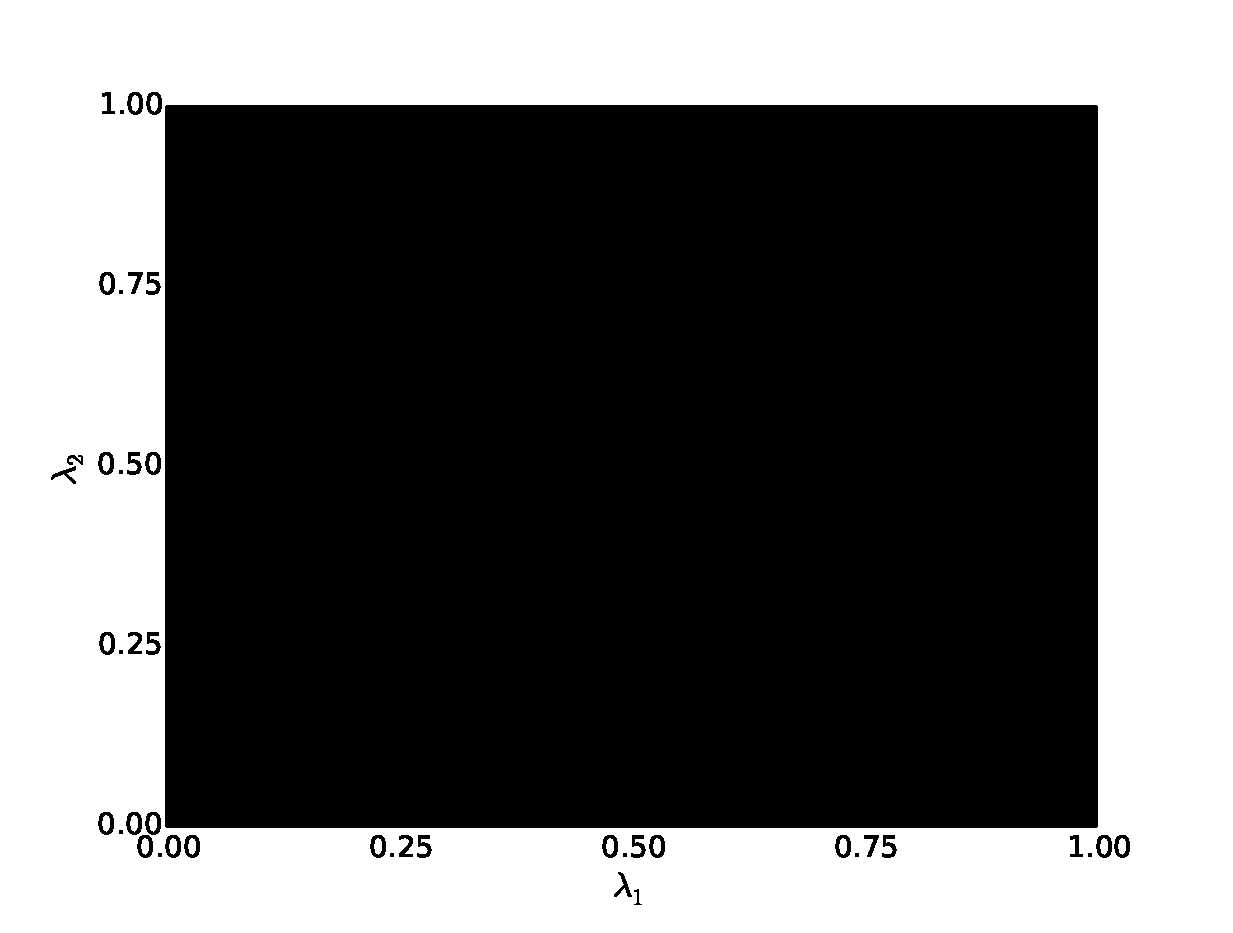
\includegraphics[width=\linewidth]{./images/voronoi_diagrams/voronoi_diagram_N25_r10}
	\end{minipage}
\caption{
Two different Voronoi partitions induced by $\nsamps_1 = \nsamps_2 = 25 $ uniform i.i.d.~random samples.
}
\label{fig:voronoi_issues}
\end{figure}


The proof of the following Lemma describes how to extend {\em any} probability measure defined on a computational algebra to the full $\sa$ $\pborel$, which we exploit in Algorithm~\ref{alg:totvar_disc}.

\begin{lem}
\label{lem:measuresets}
Let $\mu$ be a measure on $(\pspace, \BB_\pspace)$, $\set{\VV^{(j)}}_{j=1}^{\nsamps}$ be a partition of $\pspace$, and $\BB_{\pspace, \nsamps}$ the computational algebra generated by $\set{\VV^{(j)}}_{j=1}^{\nsamps}$.
Assume $\mu (\VV^{(j)}) > 0 \; \forall \; j=1,\hdots, \nsamps$.
Then, there exists a probability measure $\eta$ on $(\pspace, \BB_\pspace)$ such that $\eta(A) = \eta_\nsamps(A) \; \forall \; A\in\BB_{\pspace, \nsamps}$.
\end{lem}
In the proof below, we use $\eta_\nsamps$ and $\mu$ to construct a type of discrete Radon-Nikodym derivative of $\eta$.
This is motivated by the formal structure of solutions given by Algorithm~\ref{alg:inv_density}.
The proof of Lemma~\ref{lem:measuresets} can be found in Appendix~\ref{app:measuresets}, but the two key equations involved are reproduced here for later reference:

\begin{equation}\label{eq:finiteradon}
f_\nsamps (\param) = \sum_{j=1}^{\nsamps} \frac{\eta_\nsamps (\VV^{(j)}) }{\mu (\VV^{(j)})} \Chi_{\VV^{(j)}} (\param).
\end{equation}

Then, for any $A\in\BB_\pspace$, define

\begin{equation}\label{eq:approxmeasure}
\eta (A) = \int_A f_\nsamps (\param) \, d\mu.
\end{equation}

We note that in practice, $\Chi_{\VV^{(j)}} (\param)$ requires the use of nearest-neighbor computations, but otherwise evaluation of Eq.~\eqref{eq:finiteradon} is straightforward.


\begin{algorithm}
\DontPrintSemicolon
\caption{Total Variation Discretization}
\label{alg:totvar_disc}
Let $(\pspace, B_{\pspace, \nsamps_1}, \eta_{\nsamps_1} )$ and $(\pspace, B_{\pspace, \nsamps_2}, \eta_{\nsamps_2} )$ be given.\\

Construct $f_{\nsamps_1}$ and $f_{\nsamps_2}$ and corresponding $\eta_1, \eta_2$ using Eq.~\eqref{eq:finiteradon} and Eq.~\eqref{eq:approxmeasure}, respectively.

Use Monte Carlo sampling to approximate
$$d_\text{TV}(\eta_1, \eta_2) = \int_\pspace f_{\nsamps_1}\lam - f_{\nsamps_2}\lam \, d\mu.$$
\end{algorithm}

Since we now have a way to extend probability measures defined on $(\pspace, \BB_{\pspace, \nsamps})$ to  probability measure on $(\pspace, \BB_{\pspace})$, we can use simple Monte Carlo approximation schemes to the Total Variation distance between two probability measures defined on two separate computational algebras.
This is demonstrated in Algorithm~\ref{alg:totvar_disc}.


%%%%%%%%%%%%%%%%%%%%%%%%%%%%%%%%%%%%%%%%%%%%%%%%%%%%%%%%%%%%%%
%
\section{Numerical Results and Analysis}\label{sec:ch03-examples}
%
%
We first investigate what values of $\nsamps$ are appropriate provided the goal is to resolve $d(\PP_{\pspace, \ndiscs, \nsamps}, \PP_{\pspace, \ndiscs})$ to a desired level of accuracy so that
\begin{equation}\label{eq:newobjective}
d(\PP_{\pspace, \ndiscs, \nsamps}, \PP_{\pspace,\ndiscs}) < \tau,
\end{equation}
where $\tau$ is some designated tolerance.
%
% Recall that this discussion of error is in reference to some fixed $\qoi\in\qspace$ to which Algorithm~\ref{alg:inv_density} is applied.
% The inequality presented in Eq.~\eqref{eq:set-triangleineq} holds for probability measures induced by any map in $\qspace$, though we obscure the dependence on $\qoi$ for the time being.
% To this end, we introduce notation of the form $\PP_{\pspace, \ndiscs, \nsamps}^{\qoi}$ when we want to distinguish between measures constructed from inverting a particular map $\qoi\in\qspace$.
%
The reason for this is because the choice of $\qoi$ will influence the number of model solutions necessary to accurately solve the SIP as shown in \cite{BGE+15}.
Different choices for $\qoi$ may lead to radically different values for $\nsamps$ in order to achieve the same bound on $d(\PP_{\pspace, \ndiscs, \nsamps}, \PP_{\pspace, \ndiscs})$ as we see in the following examples.
By phrasing the analysis in terms of metrics, we are able to answer more broadly generalizable questions about error, including those regarding convergence rates and global accuracy of the estimates.


%%%%%%%%%%%%%%%%%%%%%%%%%%%%%%%%%%%%%%%%%%%%%%%%%%%%%%%%%%%%%%
We want an estimated probability measure $\hat{\PP}_\pspace$ on the parameter space to converge (with respect to the metric $d_TV$) to some reference measure $\PP_\pspace$.
This reference measure could be either some known distribution taken as truth, or another approximation deemed to be sufficiently resolved for the given application or computational budget (i.e. higher-fidelity model, mesh, or Monte-Carlo sample-size).\footnote{However, we could also choose to interrogate the push-forward measures given by propagating the $\hat{\PP}_\pspace$ and $\PP_\pspace$ forward to a data space by a QoI map and taking the distance on the resulting output space.
This would measure the ability of the maps to reconstruct the output probability measure.}

In Figure~\ref{fig:voronoi_sols}, we address the issue of comparing measures defined on two different (implicitly-defined) $\sa$s shown in Figure~\ref{fig:voronoi_issues}.
By introducing a third set against which both sample sets of size $\nsamps=50$, 

\begin{figure}[ht]
\centering
	\begin{minipage}{.275\textwidth}
		\includegraphics[width=\linewidth]{./images/voronoi_diagrams/voronoi_diagram_N25_r0_no_label}
	\end{minipage}
	\begin{minipage}{.4\textwidth}
		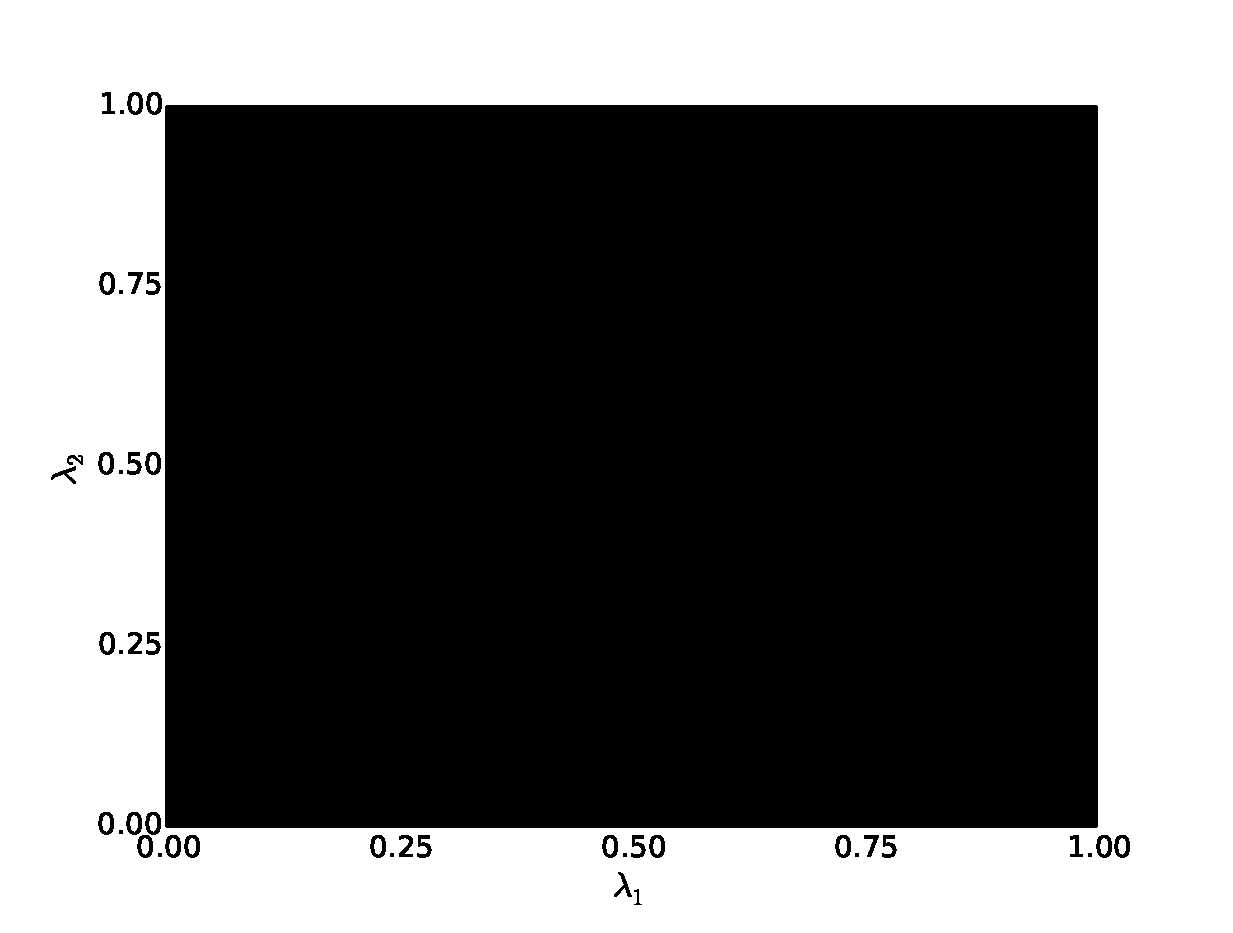
\includegraphics[width=\linewidth]{./images/voronoi_diagrams/voronoi_diagram_N500_r50}
	\end{minipage}
		\begin{minipage}{.275\textwidth}
		\includegraphics[width=\linewidth]{./images/voronoi_diagrams/voronoi_diagram_N25_r10_no_label}
	\end{minipage}
\caption{
(Left/Right): The two partitions from Figure~\ref{fig:voronoi_issues} will be projected onto a third reference partition (center), in order to compare them on a common $\sa$.
Center: A possibly over-resolved reference sample set, generated using $\nsamps = 500$ uniform i.i.d.~random samples. 
}
\label{fig:voronoi_sols}
\end{figure}


All of our experiments follow the same structure:
\begin{itemize}
\item[[0-a]] Select $\qoi\in\qspace$ and define $\PP_{\dspace_\qoi}$ as a uniform distribution centered on a reference QoI value $Q(\paramref)$ for $\paramref$ taken as the midpoint of $\pspace$. 
Note that $\PP_{\dspace_\qoi}$ is exactly discretized with $M=1$ sample, so that 
\[
P_{\pspace, 1} = P_\pspace.
\]
\item[[0-b]] Create a regular grid of samples in $\pspace=[0,1]^n$ using $N_{\text{ref},i}$ equispaced points in each dimension. 
Define $\bar{N} := \prod N_{\text{ref},i}$.
Since $n$ is small in the numerical examples shown here, we chose $N_{\text{ref},i} = 200 \; \forall \; i$ in each example.
\item[[0-c]] Use Algorithm~\ref{alg:inv_density} to construct a reference solution $\PP_{\pspace,\bar{N}}\approx \PP_\pspace$.
\item[[1]] Generate $\set{S_k^{(n)}}_{n=1}^{50}$ sets of uniform i.i.d.~random samples where $N_k = 25, 50, 100, 200, \hdots, 6400$, and $n$ represents the number of repeated trials of a sample size $N_k$.
%, constructing $\set{\set{\VVV_k^{(j)}}_{k=1}^{50}}_{j=1}^{N}$ so that when we compute Hellinger distances on the approximate measures defined on each $\set{\VVV_k^{(j)}}{j=1}{N}$, we can reduce the variance in our expected Hellinger distance values for each instance of $N$. Note that we experimented with using more trials and found the variance in expected Hellinger distances was sufficiently low with as few as twenty trials for the maps under consideration herein.
%\item[[3]] For every trial $T$ and $N$ value (including $\bar{N}$), the reference parameter $\lambda = (\lambda_1, \lambda_2) = (0.5, 0.5)$ is mapped by $Q$ to $\dspace_\qoi = Q(\pspace)$.
%\item[3] A uniform distribution with support $[Q(\lambda_1) - 0.05, Q(\lambda_1) + 0.05] \times [Q(\lambda_2) - 0.05, Q(\lambda_2) + 0.05]$ is defined on $\dspace_\qoi$, representing equal uncertainty in each component of our measured functional values.
\item[[2]] Solve the SIPs using Algorithm~\ref{alg:inv_density} to construct $\set{\PP_{\pspace,M,N}^{(n)}}_{n=1}^{50}$.
\item[[3]] Use $1E5$ i.i.d.~random samples in the Monte Carlo step of Algorithm~\ref{alg:hellinger_disc} to estimate $\set{d_H^2( \PP_{\pspace,M,N}^{(n)}, \PP_{\pspace,\bar{N}})}_{n=1}^{50}$.
\item[[4]] Average over all trials $n$ for each $N$ to estimate the {\em expected} Hellinger distance for $N$ samples and analyze convergence to $\PP_{\pspace,\bar{N}}$. 
\item[[5]] Repeat steps [0-a]--[4] for each $\qoi\in\qspace$ under consideration. 
\end{itemize}
To isolate the effect of skewness on our ability to approximate sets with finite sampling, we choose our maps so that they preserve the sizes of sets between $\pspace$ and $\dspace$ under the push-forward measure given in Eq.~\eqref{eq:dataspace_pushforward_measure}. 


\subsection{Rotational Invariance}\label{ex:rotation}
This example shows that if $\qoiA$ is defined by a rotation of $\qoiB$, then the accuracy and convergence rates of $\PP^{(a)}_{\pspace, \ndiscs, \nsamps}$ are identical to $\PP^{(b)}_{\pspace, \ndiscs, \nsamps}$.
We expect this to be true since skewness is rotationally invariant, as we summarize in the following Proposition.
\begin{prop}
The quantity $S_\qoi(\param)$ is invariant under rotations performed on $\qoi$ for any $\param$. \\
\label{prop:rot_invariance}
\end{prop}
\begin{proof}
If we apply a rotation $\qoi$, then the Jacobians $J_{\qoi, \param}$ are also subject to the same rotation at each $\param$.
Since rotations are unitary operators, the norms given in Eq.~\eqref{eq:skewness} used to define skewness are unaffected.
\end{proof}

\begin{figure}
\begin{table}[H]
\begin{tabular}{ c | c | c | c }
\nsamps & $\qoiA$ & $\qoiB$ & $\qoiC$\\ \hline \hline
$200$ & $2.18E-01$ & $1.97E-01$ & $2.19E-01$\\ \hline

$400$ & $1.60E-01$ & $1.70E-01$ & $1.51E-01$\\ \hline

$800$ & $1.09E-01$ & $1.14E-01$ & $1.09E-01$\\ \hline

$1600$ & $7.43E-02$ & $7.76E-02$ & $7.53E-02$\\ \hline

$3200$ & $5.51E-02$ & $5.53E-02$ & $5.31E-02$\\ \hline

$6400$ & $4.19E-02$ & $4.09E-02$ & $4.19E-02$\\ \hline
\end{tabular}
\end{table}

\includegraphics[width=0.45\linewidth]{./images/Plot-orth-reg_BigN_40000_reg_M_1_rand_I_100000.png}

\caption{The results of $d^2_\text{TV}(\PP_{\pspace, \ndiscs, \nsamps}, \PP_{\pspace, \bar{\nsamps}})$ for three maps generated by random rotations of orthogonal linear maps.}
\label{fig:M1orth}
\end{figure}

To demonstrate this Lemma numerically, we define the space of QoI maps $\qspace = \set{ \qoiA , \qoiB, \qoiC }$, where all three are linear maps with the same local skewness $S_\qoi (\param) = 1 \; \forall \param \in \pspace$.
The map $\qoiA$ is the identity and the other two, $\qoiB$ and $\qoiC$ are rotations of $\qoiA$ by randomly chosen angles.
Following the algorithmic outline above, we perform a convergence study to $\PP_{\pspace,\bar{\nsamps}}$ with results summarized in Figure~\ref{fig:M1orth}.
The convergence rates and expected errors in the SIPs associated with each of these maps are virtually indistinguishable.
In light of Proposition~\ref{prop:rot_invariance} and these numerical results, we conclude that the accuracy of the numerical solution to the SIP is invariant under rotations to the QoI map.

\FloatBarrier

%%%% 2D Skewness Example %%%%%% 
\subsection{Impact of Skewness on Accuracy}\label{ex:skewness}
In this example, we demonstrate the key point of this study: the magnitude of skewness between QoI impacts accuracy by orders of magnitude, and thus in optimizing the choice of a QoI map, it is in our interest to pursue the minimization of skewness. 
This is especially true in problems where the number of random samples we are permitted to use is constrained by the computational cost of model evaluations.

%Thus, any map can be thought of as a piecewise-defined linear map, and the results we present in this example, while applying to all of $\pspace$ in these cases, can be applied solely to the support of each local linear approximation.
%Capturing the geometry of sets (improving accuracy) on each of these subdomains thus guarantees a desired result on the entirety of the domain. 

To illustrate this point, we first define the linear maps 
\begin{equation}\label{eq:qmap2}
\qspace_S := \left \lbrace Q^{(s)} =  \mat{cc}{1 & 0 \\ \sqrt{s^2 - 1}& 1 } \right \rbrace_{s\in S},
\end{equation}
for $S=\set{1,2,4}$ because they allow us to control the global skewness (since it is equal to local skewness in a linear map) while preserving the measures of sets between $\pspace$ and $\dspace$. 
More specifically, the support of the solution to the SIP associated with each QoI map has equal $\mu_\pspace$-measure, which isolates the impact of accuracy solely to the skewness of the QoI map.
We show what the component row vectors of these maps in Figure~\ref{fig: skewmapvecs} and note the skewness is determined by the ratio of the magnitude of the black line to its projection onto the vertical axis (and each of these projects directly on to the unit vector).  
The skewness of these maps is given by the index $s$, so $Q^{(1)}$ is $1$, the skewness of $Q^{(2)}$ is $2$, and $S_{Q^{(4)}} = 4$.

The maps chosen for this example are expository ones that provide valuable insight despite their simplicity. 
For example, when solving many physics-based problems, local linear approximations are often used to simplify model evaluation and guide optimization procedures.


\begin{figure}[h]
	\begin{minipage}{.3\textwidth}
		\includegraphics[width=\linewidth]{./images/vector_a.png}
	\end{minipage}
	\begin{minipage}{.3\textwidth}
		\includegraphics[width=\linewidth]{./images/vector_b.png}
	\end{minipage}
	\begin{minipage}{.3\textwidth}
		\includegraphics[width=\linewidth]{./images/vector_c.png}
	\end{minipage}
\caption{(Left to right):  The component row-vectors of $Q^{(1)}$, $Q^{(2)}$, and $Q^{(4)}$. Our linear maps take $\RR^2$ to $\RR^2$ and can be visualized graphically as the component row-vectors of the matrices representing the transformation. The first row is highlighted in blue. The skewness is then simply equal to the reciprocal of the inverse sine of the angle between these vectors. }
\label{fig: skewmapvecs}
\end{figure}


\begin{figure}
\begin{minipage}{.5\textwidth}
\begin{table}[H]
\begin{tabular}{ c | c | c | c }
N & $Q^{(1)}$ & $Q^{(2)}$ & $Q^{(4)}$\\ \hline \hline
$200$ & $1.35E-01$ & $2.03E-01$ & $3.12E-01$\\ \hline 
 
$400$ & $9.96E-02$ & $1.47E-01$ & $2.15E-01$\\ \hline 
 
$800$ & $7.19E-02$ & $1.04E-01$ & $1.53E-01$\\ \hline 
 
$1600$ & $5.27E-02$ & $7.49E-02$ & $1.10E-01$\\ \hline 
 
$3200$ & $3.70E-02$ & $5.25E-02$ & $7.52E-02$\\ \hline 
 
$6400$ & $2.76E-02$ & $3.86E-02$ & $5.54E-02$\\ \hline 
\end{tabular}
\end{table}
\end{minipage}
\begin{minipage}{.45\textwidth}
		\includegraphics[width=\linewidth]{./images/Plot-reg_BigN_40000_reg_M_1_rand_I_100000}
\end{minipage}
\caption{The results of $d^2_H(\PP_{\pspace, M, N}, \PP_{\pspace,\bar{N}})$.}
\label{fig:M1_2d}
\end{figure}

We see in Figure~\ref{fig:M1_2d} that skewness has a very direct impact on the number of samples required to achieve a particular value for the Hellinger distance. 
We can see that the measure induced by $Q^{(1)}$ requires fewer than half the number of samples to be as accurately resolved as $Q^{(2)}$ does. 
The effect is even more pronounced when compared against $Q^{(4)}$.
It appears that if the ratio of skewness between two maps is 2, then the more-skewed map will require at least twice as many random samples to approximate the set on a a well-resolved discretization with the same error tolerance.

This provides a strong motivation for minimizing skewness and reinforces the results from \cite{BPW_2015}, where it was demonstrated that a similar relationship existed in the number of samples required to remove error in inverse set approximations quantified by the $\mu_\pspace$-measure of the {\em symmetric difference} of the inverse sets.




%%%% 3D Skewness Example %%%%%%

\subsection{Dependence on Dimension}\label{ex:3dmap}
We extend the numerical investigation to a parameter space of dimension three to further illustrate that these results hold as we move towards higher dimensions.
Generally, we have fewer QoI than number of uncertain model parameters, so we assume that the potential QoI maps are defined by the $2\times 3$ matrices
\begin{equation}\label{eq:qmap3}
\qspace_S := \left \lbrace \qoi^{(s)} =  \mat{ccc}{1 & 0 & 0\\ \sqrt{s^2 - 1}& 1 & 0} \right \rbrace_{s\in S}.
\end{equation}
Here, as in the previous example, the index $s$ indicates the magnitude of skewness.
Furthermore, the results of Example~\ref{ex:rotation} justify the restriction of the maps to this form since any linear map of skewness $s$ is simply a rotation of maps of this form.

%Now, the generalized contours for inverses of maps from $\RR^3 \to \RR^2$ will be isomorphic to 2\--dimensional contour events in that the inverse sets will be columns in 3\-space orthogonal to the aforemntioned plane.
%
%IMAGE DEMONSTRATING THIS WOULD HELP.
%We define
%
%which is just the map from \eqref{eq:qmap2} appended with zeros in the third column.
%We make this choice solely for convience and are justified in doing so owing to Proposition~\ref{prop:rot_invariance} and the fact of generalized contours of maps from $\RR^3 \to \RR^2$ being parallel columns.
%The rotational invariance naturally extends to the third dimension.

%We note that $\bar{N}$ is much higher since we kept the convention of 200 grid cells per dimension in our reference.
%However, we kept the same number of random samples $N$, so we should expect higher errors due to the overresolved regular grid.
%Fortunately, we find that the results still generalize.
%We present the case where $M=1$:

\begin{figure}[h]
\begin{minipage}{.5\textwidth}
\begin{table}[H]
\begin{tabular}{ c | c | c | c }
\nsamps & $\qoiA$ & $\qoiB$ & $\qoiC$\\ \hline \hline
$200$ & $2.98E-01$ & $4.18E-01$ & $5.60E-01$\\ \hline

$400$ & $2.27E-01$ & $3.27E-01$ & $4.69E-01$\\ \hline

$800$ & $1.81E-01$ & $2.70E-01$ & $3.97E-01$\\ \hline

$1600$ & $1.46E-01$ & $2.15E-01$ & $3.09E-01$\\ \hline

$3200$ & $1.15E-01$ & $1.72E-01$ & $2.44E-01$\\ \hline

$6400$ & $9.09E-02$ & $1.39E-01$ & $1.95E-01$\\ \hline
\end{tabular}
\end{table}
\end{minipage}
\begin{minipage}{.45\textwidth}
		\includegraphics[width=\linewidth]{./images/Plot-reg_BigN_8000000_reg_M_1_rand_I_100000}
\end{minipage}
\caption{The results of $d^2_H(\PP_{\pspace, \ndiscs, \nsamps}, \PP_{\pspace, \ndiscs, \bar{\nsamps}})$ for $\ndiscs = 1, \bar{\nsamps} = 8,000,000$, with $a, b, c = 1, 2, 4$.}
\label{fig:M1_3d}
\end{figure}
\FloatBarrier
In Figure~\ref{fig:M1_3d}, it appears that the effect of skewness is even more pronounced in higher dimensions, and that the number of samples required to achieve similar levels of accuracy between two maps with a ratio of skewness 2 is now quadrupled.
The analysis of \cite{BGE+15} suggested a dependence of accuracy related to the skewness raised to a power related to the dimension of the data space.

%%%%%%%%%%%%%%%%%%%%%%%%%%%%%%%%%%%%%%%%%%%%%%%%%%%%%%%%%%%%%%

% \section{Accuracy of Sample-Based Inversion}\label{sec:ch03-sample}

How does the new approach compare? What role does the KDE play in the error?
Focus on linear problems. One or two examples (perhaps use that skew-map with 1 and 2 and 4).

%%%% Sample-Based Skewness Example %%%%%%

\subsection{A Sample-Based Solution}\label{eq:sampleskew}

Here we solve the problems in Examples~\ref{ex:skewness} and~\ref{ex:3dmap}, except in the framework of the Sample-Based Inversion outlined in \ref{sec:ch02-sample}.
Effect of Skewness appears to be mitigated.
\vfill{10in}

% Total Variation\subsection{Example: Thermal Conductivity on a 1D Heat Rod}\label{ex:heat-set-sample-accuracy}

Consider the one-dimensional heat equation with homogeneous Neumann boundary conditions on the unit interval presented in \ref{ex:heat-set-sample}.


The quantities of interest we study are four point-evaluations of the state variable, at spatial location 0.25, 0.51, 0.67, and 0.98 along the rod.
Choosing any pair of them for the inversion yields six possible quantities of interest maps.
As before, we demonstrate that some choices appear to have advantages over others.

From the prior examples, we would suspect that choosing the QoI map with lower skewness results in lower Total Variations.
However in the earlier experiments we utilized maps that inverted into sets of identical size, which is not the case in this nonlinear example; each QoI map scales sets differently depending on the location in the parameter space.
To isolate this scaling effect, we attempt to compare QoIs that invert into sets of similar size \emph{on average} but have differing average skewness.

This is what motivated our specific choice of spatial locations at which to measure the state variable $T$.
Our first QoI $\qoiA$ uses measurements at 0.25 and 0.51, and has average skewness of 1.08, and our second $\qoiB$ uses measurements at 0.67 and 0.98, with average skewness 1.56.
While we would have liked to use a map with average skewness of 2 for a more similar comparison to the prior examples, this was the best range we could find where the maps inverted into sets of comparable size on average\footnote{average local scaling is $1.99$ for $\qoiA$ and $2.19$ for $\qoiB$.}.

Owing to the nonlinearity of the problem, the Total Variations between reference and estimated probability measures now have an inherent dependence on the location of the point $\param$ in the parameter space.
We ran the simulations for a regular $3\times3$ grid exploring the interior of the parameter space and present two of the nine reference points that illustrate the differences in the nonlinear case from the linear examples.
Most notably, the location of truth will impact our ability to approximate the solution to the SIP.

In the two-dimensional data spaces $\dspaceA$ and $\dspaceB$, our uncertainty is a uniform box centered at $\qoiA(\paramref)$ with side-lengths of 0.1.
When $\paramref$ is the bottom-left corner of our $3\times3$ grid, the two maps produce very different results, with $\qoiA$ outperforming $\qoiB$ in a similar manner as we saw in the linear examples (see Fig.~\ref{fig:NLbotleft}).
When $\param_{\text{ref}}$ is in the upper-center of the grid, the inverse images are similar, as shown in Fig.~\ref{fig:NLtopmid}, and so which map to use forinversion into this part of the parameter spaces is not a clear choice. We might even be tempted to use the more-skewed (on average) map since it inverts into a set with smaller support.


\begin{figure}[h]
  \includegraphics[width=\linewidth]{./images/pt0Plot-reg_BigN_40000_reg_M_1_rand_I_100000}
  \caption{Convergence in TV metric for the bottom left reference value in a 3x3 grid in $\pspace$. There is a notable difference in the accuracy of the measure recovered depending on which QoI map is used.}
  \label{fig:NLbotleft}
\end{figure}

\begin{figure}[h]
  \includegraphics[width=\linewidth]{./images/pt5Plot-reg_BigN_40000_reg_M_1_rand_I_100000}
  \caption{Convergence in TV metric for the top-middle reference value in a 3x3 grid in $\pspace$. For this value of truth, there is no distinguishable difference between the solutions that come from using either QoI map. The location in parameter space of truth will impact how sensitive experimental designs are to approximation errors in limited exploration of $\pspace$.}
  \label{fig:NLtopmid}
\end{figure}


Of the nine reference $\param$'s we studied, $\qoiA$ yielded no considerable advantage in terms of the number of samples required to approximate the inverse images in three cases (the plots were similar to that in the right of Fig.~\ref{fig:NLHD}).
In three cases, $\qoiA$ performed better than $\qoiB$, (somewhere between the two figures in Fig.~\ref{fig:NLHD}).
In two cases, $\qoiA$ performed better than  $\qoiB$, as in the left of Fig.~\ref{fig:NLHD}.
In one case (with $\param$ in the bottom right corner), the difference was even more dramatic ($\qoiA$ yielded similar Total Variations with less than a fourth the samples).

\begin{figure}
\includegraphics[width=.45\linewidth]{examples/fig_heatrod_q1/HeatrodModel--set_N50_em.png}
\includegraphics[width=.45\linewidth]{examples/fig_heatrod_q1/HeatrodModel--sample_N50_mc.png}

\includegraphics[width=.45\linewidth]{examples/fig_heatrod_q1/HeatrodModel--set_N500_em.png}
\includegraphics[width=.45\linewidth]{examples/fig_heatrod_q1/HeatrodModel--sample_N500_mc.png}

\caption{The inverse image of the reference measure for $\qoiA$ for $\nsamps = 50$ (top) and $\nsamps = 500$ (bottom). }
\label{fig:heatrod-convergence-a}
\end{figure}

\begin{figure}
\includegraphics[width=.45\linewidth]{examples/fig_heatrod_q2/HeatrodModel--set_N50_em.png}
\includegraphics[width=.45\linewidth]{examples/fig_heatrod_q2/HeatrodModel--sample_N50_mc.png}

\includegraphics[width=.45\linewidth]{examples/fig_heatrod_q2/HeatrodModel--set_N500_em.png}
\includegraphics[width=.45\linewidth]{examples/fig_heatrod_q2/HeatrodModel--sample_N500_mc.png}

\caption{The inverse image of the reference measure for $\qoiB$ for $\nsamps = 50$ (top) and $\nsamps = 500$ (bottom). TK - need to remark about how this map may be more precise but it makes it harder to identify the set that contains truth when few model evaluations are available to us (low $\nsamps$). }
\label{fig:heatrod-convergence-b}
\end{figure}


These results motivate further study into utilizing different QoI maps (perhaps some of those other four combinations available to us in this example) depending on where the samples came from in the parameter space.
In general, we saw in this example that given that two maps invert into sets of similar size on average, using the one with lower skewness results in less samples required to accurately approximate the inverse image.
The maps we used had average skewnesses that differed by 0.5 (instead of by 1), and the trend from the linear examples still held in significant portions of the parameter space.

% \FloatBarrier
%
% \subsection{Exponential Decay: Initial Condition and Rate}\label{ex:decay-set-sample-accuracy}

\begin{figure}[h]
\begin{minipage}{.4\textwidth}
\includegraphics[width=\linewidth]{examples/fig_decay_q1/DecayModel--set_N50_em.png}
\includegraphics[width=\linewidth]{examples/fig_decay_q1/DecayModel--set_N500_em.png}

\includegraphics[width=\linewidth]{examples/fig_decay_q2/DecayModel--set_N50_em.png}
\includegraphics[width=\linewidth]{examples/fig_decay_q2/DecayModel--set_N500_em.png}
\end{minipage}
\begin{minipage}{.4\textwidth}
\includegraphics[width=\linewidth]{examples/fig_decay_q1/DecayModel--sample_N50_mc.png}
\includegraphics[width=\linewidth]{examples/fig_decay_q1/DecayModel--sample_N500_mc.png}

\includegraphics[width=\linewidth]{examples/fig_decay_q2/DecayModel--sample_N50_mc.png}
\includegraphics[width=\linewidth]{examples/fig_decay_q2/DecayModel--sample_N500_mc.png}
\end{minipage}

\caption{The inverse image of the reference measure for $\qoiA$ (top half) and $\qoiB$ (bottom half). }
\label{fig:decay-convergence}
\end{figure}

With these nonlinear cases, we find that taking an ``on average'' approach is inefficient, as there can be dramatic differences in the geometric properties of the inverse images in the parameter space depending on the location.
These results motivate further study into utilizing different QoI maps (perhaps some of those other four combinations available to us in this example) depending on where the samples came from in the parameter space.
In general, we saw in this example that given that two maps invert into sets of similar size on average, using the one with lower skewness results in less samples required to accurately approximate the inverse image.
The maps we used had average skewnesses that differed by 0.5 (instead of by 1), and the trend from the linear examples still held in significant portions of the parameter space.


\section{Conclusions}
In this chapter we reviewed the skewness property of QoI maps and demonstrated that for solutions to the SIP, maps which exhibit lower values of skewness exhibit lower overall finite-sampling approximation error against a reference solution.
We saw that the solutions are invariant to transformations such as rotation (which also holds for translations).
The latter observation may aid in the selection of optimal maps (i.e., one can disregard the direction of the maps' contours and focus solely on the angles among the generalized contours).
In the following chapter, we show how vector-valued QoI maps such as those in Chapter~\ref{chapter:mud} constructed from data relate to the geometry of the resulting data-spaces and subsequently impacts the solutions to the SIP.
We demonstrate that even a basic awareness and consideration of skewness can aid in the construction of maps which are more informative and thus increase the precision of parameter estimates.

\FloatBarrier

%\chapter{\uppercase{Extensions and Applications of MUD Points and Skewness Analysis} \label{chapter:vector-valued}}


\section{Extension to Vector-Valued QoI Maps}
The examples in Sections~\ref{subsec:ode-example} and \ref{subsec:pde-example} motivate the use of a data-constructed QoI in order to incorporate an arbitrary number of measurements in a system into a scalar-valued map.
These examples were chosen so that $\text{dim}({\Lambda}) = 1$ for simplicity and to establish a baseline for convergence results.
The linear examples in Section~\ref{subsec:high-dim-linear-example} demonstrate that the DCI framework maintains the accuracy of least-squares while incorporating initial beliefs for higher-dimensional linear maps.
In those examples, we showed that our ability to resolve a true parameter improved as the gap between input dimension and operator row-rank shrunk.

The rank-deficiency of an operator can be attributed either to ill-conditioning of an operator $A:P\to P$, or when $P>D$ for a full-rank $A:P\to D$.
In scenarios where $S>P$ observations are available, we are motivated to somehow leverage the form of Eq.~\eqref{eq:qoi_WME} to construct a vector-valued version incorporating subsets of $S$ for each component.
For example, a system for which spatial measurements are available over time may motivate constructing a scalar-valued WME map for each spatial location.
If distinctly different observable quantities are available (ones perhaps with different physical units), then these may be collapsed into each component of the map.

The discussion of how to optimally construct such maps is beyond the scope of this work, and would need to take into account nuances involving measurement sensitivities and address combinatorial design-spaces.
However, we summarize that the extension of the equations presented in Section~\ref{sec:MUD_analysis} follows directly by constructing the resultant $1\times P$ matrices $A$ and scalar-valued $b$ for each component and then stacking them to form a $D\times P$ system, where we are motivated to minimize $P-D$.

%%%%%%%%%%%%%%%%%%%%%%%%%%%%%%%%%%%%%%%%%%%%%%%%%%%%%%%%%%%%%%%%%%%%
%%%%%%%%%%%%%%%%%%%%%%%%%%%%%%%%%%%%%%%%%%%%%%%%%%%%%%%%%%%%%%%%%%%%

\subsection{A Vector-Valued QoI Map}
In the previous example, we presumed a fair bit of prior knowledge about the structure of $g$ being a sine curve; we only had to estimate a scaling coefficient for it.
To demonstrate the use of the WME QoI in solving inverse problems in higher dimensions, we set up the following series of examples in the same spirit as the former, presuming less about $g$ than before.
Suppose we know that $g$ is negative and bounded below by $-4$, and we pursue estimating it by first placing two knots on the interior of the domain of $g$ and estimating its value at these points.
This gives us a parameter space of $\pspace = [-4, 0]$, and we choose a polynomial function $g$ which exhibits similar behavior to the former $\sin$ curve, but without the symmetry about $x_2=0.5$, and scale it so that it takes a minimum at the same value as before (at $-3$).
Over this space we will assume a uniform density again.
We selected $g(x) = \alpha x_2^2 (x_2 - 1)^5$, with $\alpha$ chosen to satisfy the aforementioned design specification (so that $g(x)=-3$ for $x=(0,\frac{2}{7})$).

Our first two knots will be the equispaced points $x = (0,\frac{1}{3}), (0,\frac{2}{3})$, and the family of functions that this spans is visually illustrated in the left half of Figure~\ref{fig:pde-highd-initial}, alongside the true function and the associated piecewise--linear that comes from interpolating the true $g$.
The rest of the problem setup will be kept the same as the previous example, except that instead of $N=10,000$ parameter space samples, we use $1,000$.
The reason for this is that we will not be doing the same convergence studies, so we are less interested in exhaustively exploring $\pspace$ than demonstrating that our method can handle a wider variety of inverse problems than the previous examples may suggest.


\begin{figure}
\centering
  \includegraphics[width=0.475\linewidth]{figures/pde-highd/pde-highd_init_D2.png}
  \includegraphics[width=0.475\linewidth]{figures/pde-highd/pde-highd_init_D5.png}
\caption{
One thousand initial parameter samples (our model evaluation ``bugdet'') were used to estimate $g$, constructed by taking independent uniform samples from $[-4, 0]$ for each direction are shown in gray. (Left): Two-knot problem. (Right): Five-knot problem.
}
\label{fig:pde-highd-initial}
\end{figure}

\subsubsection{A Scalar-Valued QoI Map}

Our first inverse problem will involve solving the SIP with the same scalar-valued QoI map constructed by incorporating all the measurements into \eqref{eq:qoi_WME}, and to give the reader a sense of the ability for this ``basis'' to match the one-hundred measurements used for inversion, we plot the best match of our thousand parameter samples with respect to these measurements in purple in the top half of Figure~\ref{fig:pde-highd-2d-scalar-mud}.
There, we also plot the closest match to the interpolating piecewise-linear function in green, and note that we have a near-identical match among our thousand parameter samples, though the best predictor of the data we collected is a different sample.
We are curious which of these two functions the MUD will more closely resemble.
The residual Q-Q plots for the two functions are shown to illustrate the differences in misfit to provide an alternative view to the goodness-of-fit.


\begin{figure}
\centering
  \includegraphics[width=0.95\linewidth]{figures/pde-highd/pde-highd_proj_D2.png}
  \includegraphics[width=0.95\linewidth]{figures/pde-highd/pde-highd_pair_D2-1_m100.png}
\caption{
}
\label{fig:pde-highd-2d-scalar-mud}
\end{figure}

In the bottom half of \ref{fig:pde-highd-2d-scalar-mud}, we show the MUD solutions arising from twenty trials using different observations of noise.
Of particular interest is that the solutions seem to discover one of two types of explanations for the data, seemingly unable to decide which half of the domain represents a better estimate of $g$'s minimum value.
As mentioned, this set of solutions comes from collapsing all hundred measurements into a scalar--valued QoI map, which negatively impacts our ability to identify the parameter in the problem, since our SIP is now $2\rightarrow 1$.
[TK - cite Troy's result about dimensions from AWR paper] implies that we have an incentive to construct maps which ``close the gap'', so to speak, between input and output dimension, to fully leverage the geometry of available information.
This can be seen in the contour structure of the updated density samples plotted in red in \ref{fig:pde-highd-2d-example}.


\FloatBarrier
\subsubsection{Some (Options for) Vector-Valued QoI Maps}

Suppose that instead of constructing a scalar--valued QoI map, we used the form of \eqref{eq:qoi_WME} to construct a map with two components, yielding a $2 \rightarrow 2$ SIP instead.
Would such an approach provide any tangible benefit for resolving the uncertainty in our true function $g$?
To explore this question, we propose two relatively uninteresting methods for splitting our hundred measurements in to two sets which will be used to construct each component of the map according to \eqref{eq:qoi_WME}.
Both are shown in the top half of Figure~\ref{fig:pde-highd-2d-geometry}, and represent a bisection through $\Omega$ vertically and horizontally.

\begin{figure}
\centering
  \includegraphics[width=0.475\linewidth]{figures/pde-highd/pde-highd_sensors_D2.png}
  \includegraphics[width=0.475\linewidth]{figures/pde-highd/pde-highd_sensors-alt_D2.png}
  \includegraphics[width=0.95\linewidth]{figures/pde-highd/pde-highd_geom_D2.png}
\caption{
(Bottom): The vector-valued QoI map is constructed for all $N=10,000$ parameter evaluations and the two resulting vectors are plotted against one another for both methods of partitioning $\Omega$.
}
\label{fig:pde-highd-2d-geometry}
\end{figure}

There are now two QoI maps under consideration, which should we use?
Before solving an inverse problem, there are a-priori analysis that can be performed that can provide heuristics to help address these questions.
We first evaluate our thousand parameter samples through each of these maps and inspect the two-dimensional scatter-plots to build intuition about the underlying geometry induced by these maps.
We repeat this process for three subsets of the measurements (using the first samples in each half of $\Omega$ according to the random index assigned to them), and demonstrate the two resulting sets of relationship in the bottom half of Figure~\ref{fig:pde-highd-2d-geometry}.
This figure also shows the associated designs against the noisy response surface as a backdrop.

\subsubsection{An Aside for Geometric Considerations}

First, we note that the inclusion of more data points has the effect of dilating (and to some extent rotating) the induced data space for both QoI maps.
The geometric implication of this in the context of the chosen form of the QoI map has an interesting consequence.
Recall that the observed distribution remains a standard Gaussian, regardless of the number of data points used to construct the map.
In two dimensions, this observed distribution becomes a multivariate normal distribution instead, which can be visually thought of as a circular ``target'' located in the middle of each of the scatter-plots in Fig. \ref{fig:pde-highd-2d-geometry}.
As more measurements are incorporated, the size of that target relative to the rest of the space becomes increasingly small since the data manifolds dilate.
If the reader would indulge the author in another metaphor, it is akin to finding the same needle in larger piles of hay.
More is asked of the solution to the SIP, since there are more measurements with which the model must agree.

The second implication of the two ways in which the maps can be formed is more visually evident, as the two quantities of interest that arise from a vertical bisection of $\Omega$ are nearly perfectly correlated.
The two maps are presenting almost the same information (the shapes are very slim parallelograms), and so we fundamentally can already expect there to be very little difference between MUD points arising from using this map when compared to using the scalar--valued map.
Particularly since the observed distribution is radially symmetric, this problem\---while technically two-dimensional\---appears to be one-dimensional.

By contrast, the map induced by a horizontal split (bottom left of Fig. \ref{fig:pde-highd-2d-geometry}) provides new information in each component.
While there is some correlation (the manifolds are not rectangular), a far greater proportion of samples will fall within the practical support of the observed distribution, which qualifies them as possible solutions to the SIP.
More information is learned with the inclusion of each component using this design than would be with the vertical split.

To this end, for the sake of brevity, we focus our attention on comparing the horizontal vector--valued QoI map to the scalar one, and note that a more fulfilling discussion of constructing QoI maps that induce desirable geometric properties is of interest for future work.
For the remainder of this example, the ``vector--valued'' map will refer to the the one which is split horizontally, and we note that this design, while not having any guarantees of optimality for precision or accuracy's sake, at least respects the flow of information in the system being studied.
Since $\param$ is parameterizing the left Neumann boundary condition, information about its state flows from left to right in the horizontal direction.



\FloatBarrier
\subsubsection{Comparing Solutions}

We turn the reader's attention to Figure~\ref{fig:pde-highd-2d-example}, which illustrates an example MUD solution for both the scalar-- and vector--valued QoI maps.
The predicted response surfaces are shown at the top, and the associated functions and residual plots are below it.
In this particular instance, it appears that the vector-valued MUD solution does a better job capturing the qualitative behavior of $g$; the difference in the residuals is less pronounced.
Both solutions manage to capture some general behavior of the true function, but to better understand the differences in the two solutions, we need instead to look at the set of probable samples, not only the most likely among them.

\begin{figure}[htbp]
\centering
  \includegraphics[width=0.95\linewidth]{figures/pde-highd/pde-highd_surf_exmud_D2_m100.png}
  \includegraphics[width=0.6\linewidth]{figures/pde-highd/pde-highd_comp_exmud_D2_m100.png}
\caption{
100 measurements
}
\label{fig:pde-highd-2d-example}
\end{figure}


This is what is shown at the bottom of Fig.~\ref{fig:pde-highd-2d-scatter}: we normalize our ratio pdf evaluations and plot the samples that exceed two thresholds, numerical zero (left), and $1/N$ (right) to give some sense of samples that may come from accept/reject algorithms (since our initial was uniform).
Both scatter-plots exhibit the same geometry, appearing to trace a band through the parameter space.
Fundamentally, at first glance at the left figure, it is already apparent that half of $\Lambda$ has been ruled out, and that the correlation structure between the two knots has been discovered.
The vector--valued samples, however, cluster more tightly around the optimal samples (the ``projection'' here refers to the sample which minimizes the 2-norm to the noiseless data).
The incorporation of two directions instead of one whittles away more of the parameter space as being less relatively likely.
If we were to perform accept/reject, the resulting set would be fairly well constrained to the upper-lefthand corner of the two-dimensional parameter space.

\begin{figure}[htbp]
\centering
  \includegraphics[width=0.45\linewidth]{figures/pde-highd/pde-highd_update_scatter_D2_t1-0E-16.png}
  \includegraphics[width=0.45\linewidth]{figures/pde-highd/pde-highd_update_scatter_D2_t1-0E-03.png}
\caption{
100 measurements
}
\label{fig:pde-highd-2d-scatter}
\end{figure}

To rule out the possibility that our one updated density / MUD point was luck, we again re-solve our SIP for twenty different realizations of noise to pollute our hundred measurements, and show the resulting solutions for the first twenty and all hundred being used to construct the vector--valued map.
The resulting functions that are induced by these MUD points are shown in Fig.~\ref{fig:pde-highd-2d-vector-mud}, and we note that solutions are no longer are considering the possibility of the minimum value of $g$ being at the wrong knot point as we saw in Fig.~\ref{fig:pde-highd-2d-scalar-mud}, even when only twenty total data points are used to construct $Q$.
By the time all hundred measurements are incorporated, the MUD solutions appear to be tracing out curves between the projection function and the interpolant function, a far more accurate set of predictions than those from the scalar--valued map.

\begin{figure}[htbp]
\centering
  \includegraphics[width=0.6\linewidth]{figures/pde-highd/pde-highd_pair_D2-2_m20.png}
  \includegraphics[width=0.6\linewidth]{figures/pde-highd/pde-highd_pair_D2-2_m100.png}
\caption{
(Top): When vectorizing our QoI map, we find that we are able to achieve more accuracy with fewer measurements. Here, we see far less variation in MUD solutions than in the bottom of Fig.~\ref{fig:pde-highd-2d-scalar-mud}.
(Bottom): When all 100 measurements are incorporated
}
\label{fig:pde-highd-2d-vector-mud}
\end{figure}

How we incorporate the available data has a dramatic impact on our ability to reduce uncertainty in the parameter space.
We attempt to illustrate this by requesting the reader juxtapose figures of the initial samples in \ref{fig:pde-highd-initial} to those in \ref{fig:pde-highd-2d-scalar-mud} and \ref{fig:pde-highd-2d-vector-mud}.
To better quantify the differences, it is more rigorous to study how close we are to $g$ (in function space).
Since the approximation $\hat{g}$ that arises from evaluating the MUD point is piecewise-linear, and $g$ is continuous, we use the knot points and the trapezoidal rule to approximate the $L^2$ norm of $\abs{g - \hat{g}}$ (using {\tt scipy}), and plot the resulting histograms for the scalar- and vector-valued $\param$s whose relative ratios exceeded a threshold, and compare them against samples from the initial density, and show the result in Figure~\ref{fig:pde-highd-2d-hist}.


\begin{figure}[htbp]
\centering
  \includegraphics[width=0.675\linewidth]{figures/pde-highd/pde-highd_hist_D2_t5-0E-01}
\caption{
Histograms comparing initial samples with the highest probabilities (relative ratio $> 0.5$).
}
\label{fig:pde-highd-2d-hist}
\end{figure}

In \ref{fig:pde-highd-2d-hist}, the histograms have been normalized for comparison, and while the scalar--valued map still does reduce the uncertainty that we started with in our initial density.
The multi-modal nature of this plot shows a lack of resolution that is not experienced at all by the vector--valued solution.
This multi-modal density of probably samples corresponds to the two types of solutions we saw in Figure~\ref{fig:pde-highd-2d-scalar-mud}.
Both QoI maps solve a stochastic inverse problem, but the latter is more respectful of the geometry of the response surface, and so is able to learn significantly more, and bring us modelers far closer to the true function $g$.


%%%%%%%%%%%%%%%%%%%%%%%%%%%%%%%%%%%%%%%%%%%%%%%%%%%%%%%%%%%%%%%%%%%%
%%%%%%%%%%%%%%%%%%%%%%%%%%%%%%%%%%%%%%%%%%%%%%%%%%%%%%%%%%%%%%%%%%%%
\FloatBarrier
%%%%%%%%%%%%%%%%%%%%%%%%%%%%%%%%%%%%%%%%%%%%%%%%%%%%%%%%%%%%%%%%%%%%
%%%%%%%%%%%%%%%%%%%%%%%%%%%%%%%%%%%%%%%%%%%%%%%%%%%%%%%%%%%%%%%%%%%%
\subsection{Extension to Higher Dimensions}

Suppose now that an eager experimenter decided to start with a five--dimensional problem (five knots instead of two), trying to accomplish greater granularity in the ability to estimate $g$, and imposes the same type of uniform initial in each direction, yielding a parameter space of $\Lambda = [-4, 1]^5$.
In Figure~\ref{fig:pde-highd-initial}, we show what such initial functions would look like, and note that many of them appear to exhibit fluctuating behavior for which the mesh ($36\times36$) being used to solve the problem, would not be fine enough to resolve.
In many senses, this choice of initial density induces a lot of noise into the SIP we are hoping to solve, since ``common sense'' from a modeler's perspective may be able to rule out zig-zag functions from wasting model-evaluation budget, which we retain at the same $N=1000$ samples as in the previous 2-D problem.
To get a sense of what the best possible representations in this peculiar choice of ``basis'' could be, we again find the closest match to the interpolant and to the data and plot them alongside residuals in Figure~\ref{fig:pde-5d-proj}.

\begin{figure}[htbp]
\centering
  \includegraphics[width=0.675\linewidth]{figures/pde-highd/pde-highd_proj_D5}
\caption{
}
\label{fig:pde-5d-proj}
\end{figure}

Observe that in Figure~\ref{fig:pde-5d-proj}, both the closest fit in parameter and measurement space fail to resolve the true function behavior at $\lambda_5$ (the interpolating piecewise--linear is shown for reference), and both place a minimum at $\lambda_2$.
The plot here is in some sense, the best that can be solved for with this design, and is helpful for comparing against our MUD solutions.
Of particular interest here is to note also is that both functions under-estimate $g$ at $\lambda_2$ by a large margin.
Nevertheless, we pursue the solution for demonstration purposes and solve the SIP for both scalar-- and vector--valued QoI maps, the latter constructed with horizontal bands shown in the bottom left of Figure \ref{fig:pde-highd-5d-example}.

\begin{figure}[htbp]
\centering
  \includegraphics[width=0.95\linewidth]{figures/pde-highd/pde-highd_surf_exmud_D5_m100}
  \includegraphics[width=0.35\linewidth]{figures/pde-highd/pde-highd_sensors_D5}
  \includegraphics[width=0.6\linewidth]{figures/pde-highd/pde-highd_comp_exmud_D5_m100}
\caption{
(Top): Layout for 5-D vector--valued map and comparison of the two MUD solutions in parameter space.
(Bottom): The response surfaces predicted by the two QoI maps alongside the noisy response surface that generated the simulated collected data.
}
\label{fig:pde-highd-5d-example}
\end{figure}

In Figure~\ref{fig:pde-highd-5d-example}, the scalar-- and vector--valued MUD solutions are shown for the noisy surface plotted in the top-center, with associated predicted response surfaces flanking it.
In the bottom-center plot, we can see that the scalar-valued MUD happens to completely misidentify the location of $g$'s minimum value, but the vector-valued QoI is able to resolve the behavior much better.
In Figure~\ref{fig:pde-highd-5d-mud} we plot the results from twenty repeated trials (perturbations of noise) when using all hundred measurements, and observe the same difference in going from scalar-- to vector--valued solutions for the five--dimensional example that we saw in two dimensions in \ref{fig:pde-highd-2d-scalar-mud}.

\begin{figure}[htbp]
\centering
  \includegraphics[width=0.95\linewidth]{figures/pde-highd/pde-highd_pair_D5-1_m100}
  \includegraphics[width=0.95\linewidth]{figures/pde-highd/pde-highd_pair_D5-5_m100}
\caption{
(Top): Scalar-valued solutions.
(Bottom): Vector-valued solutions.
}
\label{fig:pde-highd-5d-mud}
\end{figure}

By increasing the number of quantities of interest used, more directions of uncertainty are resolved in the parameter space.
Since any solution in the equivalence class is a valid one for the SIP, the scalar-valued solutions are much more sensitive to the noise, and so the solutions often appear to identify functions with a minimum on the wrong half of the domain.
In Figure~\ref{fig:pde-highd-5d-mud}, the scalar-valued QoI is unable to differentiate between resolving residual discrepencies in different locations in $\Omega$.
By contrast, the vector-valued QoI is constructed with respect to the flow of information in the system, and so many more of the twenty trials land closer to the true minimum value of $g$.
The solutions for the vector-valued approach instead explore the available knots (at $x_2=1/6$ and $1/3$), nearest the actual minimum value of $2/7$ instead, a much more valuable area of $\Lambda$ to explore.

Perhaps unsurprisingly given the poorly-designed initial density, our MUD solutions still do not really trace out the interpolant that we hope it should in order to approximate $g$.
At the very least, we would hope to accurately estimate the location and value of $g$'s minima.
Recall that we have already solved a two-dimensional version of this problem, which could have been used to inform a much smaller region of two of the five directions to explore.
Let us see what would happen if our initial density was constructed with more care (without needing to use any model evaluations), since we saw from earlier examples that if DCI is initialized at a good initial mean, it has a chance of outperforming even least-squares in resolving discrepency in truth.

%%%%%%%%%%%%%%%%%%%%%%%%%%%%%%%%%%%%%%%%%%%%%%%%%%%%%%%%%%%%%%%%%%%%
%%%%%%%%%%%%%%%%%%%%%%%%%%%%%%%%%%%%%%%%%%%%%%%%%%%%%%%%%%%%%%%%%%%%

\subsection{Alternative Experimental Approach}

[TK - Now we're tying back into the OED discussion]

As we proceed from two to five dimensions, being weary of the fact that we are fighting against the curse of dimensionality, we want to be more intelligent with our specification of an initial density.
Let us take a look at the samples that show up in black on the bottom-right of Figure~\ref{fig:pde-highd-2d-example} from a different perspective.
Instead of looking at high-probability samples as locations in $\Lambda$, let us inspect them as a family of functions that are defined on the unit interval and use the envelope curves they sweep out to inform the specification of a better initial density; consider Figure~\ref{fig:pde-highd-5d-study}.

\begin{figure}[htbp]
\centering
  \includegraphics[width=0.675\linewidth]{figures/pde-highd/pde-highd-alt_initial_D5_m100.png}
\caption{
}
\label{fig:pde-highd-5d-study}
\end{figure}

The samples whose relative ratios exceeded $1/1000$ sweep out a family of curves that can be used to estimate bounds not only on $\lambda_2$ and $\lambda_4$ (the previous $\lambda_1$ and $\lambda_2$ from the 2-D problem)\---which exhibit correlation structure that we will turn to momentarily\---but also on the remaining three knots.
To form the intervals shown in orange in Fig.~\ref{fig:pde-highd-5d-study}, we take the upper and lower bounds of the curves passing through the vertical lines drawn at the three new knot values.
To be conservative, we multiply our lower bound by $1.2$ and the upper by $0.8$ (we are still more than halving the interval-length in each direction as compared to the previous 5-D problem).
(Alternatively, one could establish a lower tolerance for accepting likely samples and avoid the multiplication factor, but the authors enjoyed the connection to accepted samples from the updated density).

\subsubsection{A better initial density}
For the two directions remaining, we want to capture the correlation structure that we were able to visually identify in Fig.~\ref{fig:pde-highd-2d-example} and impose something uniform-like on it.
To achieve this, we perform a singular-value decomposition on the likely samples from the \emph{scalar}--valued 2-D solution, since there are so many more samples (it was found to better characterize the direction of the equivalence class, suggesting perhaps a justifiable use for solving the problem with it in such cases).

The singular vectors are used to transform the vector-valued samples, and a uniform sampling is performed over the rectangular bounding box for these points, shown in the center of Figure~\ref{fig:pde-highd-2d-study}.
These generated samples, however, leave $\Lambda$ when transformed back to their native space, as seen in the left panel.
To ameliorate this problem, we instead perform sampling in a while-loop, sampling from this uniform box and rejecting any that would get mapped back outside $\Lambda$.


\begin{figure}[htbp]
\centering
  \includegraphics[width=0.95\linewidth]{figures/pde-highd/pde-highd-alt_initial_D2_m100}
\caption{
Generating proposal samples for the two directions informed by solving the 2-D inverse problem, aided by singular-value decompositions and a basic ad-hoc sampling procedure.
}
\label{fig:pde-highd-2d-study}
\end{figure}

Furthermore, note that in the center of the Fig~\ref{fig:pde-highd-2d-study}, there are corner-regions of the space we want to avoid wasting samples on as well, so we reject samples that have squared two-norm greater than $0.05$ from their nearest vector--valued sample.
This sampling procedure produces the set shown in orange on the right side of the figure (ten thousand shown to demonstrate coverage).
In a sense, we wanted to quickly define a computational open cover for the relatively high-probability samples.
We keep one thousand of these 2-D samples, and join them with the three independent uniform sample sets of the same size taken from the intervals in Fig.\ref{fig:pde-highd-5d-study} to form our new initial sample set, the functions from which generate the curves shown in Figure~\ref{fig:pde-highd-5d-init}.

\begin{figure}[htbp]
\centering
  \includegraphics[width=0.675\linewidth]{figures/pde-highd/pde-highd_init_D5-alt}
\caption{
Initial density constructed for the second attempt at the five--dimensional inverse problem, with the structure of solutions learned from the 2-D example incorporated into the selection of bounds in each direction.
}
\label{fig:pde-highd-5d-init}
\end{figure}

These curves, especially when contrasted to those in Fig.~\ref{fig:pde-highd-initial}, represent a far more reasonable set of possibilities, exhibiting none of the erratic roughness that was seen in the first attempt at a five--dimensional initial density.
We note that such considerations of smoothness could be avoided by parameterizing $g$ with a basis of some sort, but that problem is beyond the scope of this already lengthy work.
Another possible improvement would be to incorporate the correlation structure that is present in the three other directions, derivable from a similar SVD-based analysis of the interpolation of the 2-D predictions through the new knot locations, but that would require more visual exploration than the authors deem worthwhile to demonstrate the point they are trying to make.

\begin{figure}[htbp]
\centering
  \includegraphics[width=0.95\linewidth]{figures/pde-highd/pde-highd_surf_exmud_D5-alt_m100.png}
  \includegraphics[width=0.9\linewidth]{figures/pde-highd/pde-highd-alt_comp_exmud_D5_m100.png}
\caption{
100 measurements for the revised five--dimensional problem yield substantially better estimates in the eyeball norm.
}
\label{fig:pde-highd-5d-alt-example}
\end{figure}


\subsubsection{Moving to Five Dimensions with more caution}

We now come to the solutions that arise from solving the same five--dimensional inverse problem of interpolating the values of $g$ through equispaced knot points, with both types of maps, in Figure~\ref{fig:pde-highd-5d-alt-mud}.
The difference in comparison to the example solutions in Fig.~\ref{fig:pde-highd-5d-mud} is stark: no longer are the solutions dramatically under-estimating the local minimum of $g$.
To the extent to which they fail to adequately to do is due to the insufficient resolution of five knot points; both scalar-- and vector--valued solutions identify the same knot as being the likely minimum, and the latter solution estimates the minima well (horizontal line drawn for reference) in the bottom-right plot.

Once again, we repeat the experiment twenty times to better understand the differences in the solutions relative to possible noise that polluted our measurements.
We are able to notice some interesting patterns by looking at the curves on the left side of Figure~\ref{fig:pde-highd-5d-alt-mud}.
First, we note that going from scalar-- to vector--valued resolves a significant amount of uncertainty in $\lambda_2$, $\lambda_3$, and $\lambda_4$, namely the QoI map appears to stop considering curves which do not have a sufficiently low minimum value.
Second, while the vector--valued MUD solution curves appear to capture the general characteristics of $g$ well, a number of them under-estimated the value at $\lambda_5$ quite severely relative to the true value (near zero), which we saw in Figure~\ref{fig:pde-highd-5d-mud} as well.

\begin{figure}[htbp]
\centering
  \includegraphics[width=0.95\linewidth]{figures/pde-highd/pde-highd_pair_D-alt-5-1_m20.png}
  \includegraphics[width=0.95\linewidth]{figures/pde-highd/pde-highd_pair_D-alt-5-5_m20.png}
\caption{Compared to before, we're doing much better, even with less data incorporated into our QoI maps.}
\label{fig:pde-highd-5d-alt-mud-20}
\end{figure}

\begin{figure}[htbp]
\centering
  \includegraphics[width=0.95\linewidth]{figures/pde-highd/pde-highd_pair_D-alt-5-1_m100.png}
  \includegraphics[width=0.95\linewidth]{figures/pde-highd/pde-highd_pair_D-alt-5-5_m100.png}
\caption{
(Top): Scalar-valued solutions for alternative approach to the five-dimensional problem.
(Bottom): Vector-valued solutions.
Because we began with a better choice of initial density, both QoI maps resolve the residuals similarly (bottom-left), and produce qualitatively similar estimates of the response surface. We attribute this to the fact that the vector--valued samples were used to bound the space, but note the direction was informed by the scalar--valued samples.
}
\label{fig:pde-highd-5d-alt-mud}
\end{figure}
\FloatBarrier


\subsubsection{Demonstration of Reduction in Uncertainty}

As a final note on this experiment, we contrast the resulting $L^2$-errors to $g$ \footnote{derived from computational approximation with the trapezoidal rule} of these MUD solutions, to the previous two examples in Figure~\ref{fig:pde-highd-5d-hist}, to show a lineage of learning, so-to-speak.
With each successive problem, our uncertainty is reduced and our MUD solutions lower in variance and increase in accuracy.
Note that they appear to be moving towards a value away from zero, which represents a fixed bias (five equispaced knots can only approximate this $g$ so well).

\begin{figure}[htbp]
\centering
  \includegraphics[width=0.675\linewidth]{figures/pde-highd/pde-highd_hist_D5_t5-0E-01}
\caption{
Comparison of the 2D initial errors to the 5D ones, as well as the reduction of uncertainty that solving a SIP problem for each provides.
}
\label{fig:pde-highd-5d-hist}
\end{figure}

\FloatBarrier


% ---------------------------------------------------------------------------- %
\renewcommand\bibname{REFERENCES}
\singlespacing

\nocite{*}
\bibliographystyle{ucdDissertation}
\bibliography{references,r-references}

\doublespacing

% ---------------------------------------------------------------------------- %
% had to do some TOC shenanigans, so please use the ucdappendix command instead
% of regular old \appendix
\ucdappendix

\chapter{\uppercase{Abbreviations and Notation} \label{appendix-notation}}

\section{Abbreviations}

\begin{description}[leftmargin=!,labelwidth=0.5in,font=\normalfont]
	\item 
\end{description}


\section{Mathematical Notation}
\begin{description}[leftmargin=!,labelwidth=0.5in,font=\normalfont]
	\item 
\end{description}


\subsection{General Notation}

\begin{description}[leftmargin=!, labelwidth=0.7in]
  \item[$x$]             italicized, Roman or Greek letter, denotes a scalar values 
  \item[$\bs{x}$]        italicized, bold, lowercase Roman or Greek letter, denotes a column vector or set.
  \item[$\bs{X}$]        italicized, bold, uppercase Roman or Greek letter, denotes a matrix or set.
  \item[$\card{\bs{x}}$] cardinality, number of elements, of the vector or set $\bs{x}$ 
  \item[$x \in (a, b)$]  the value $x$ is within the interval such that $a < x < b$
  \item[{$x \in (a, b]$}]  the value $x$ is within the interval such that $a < x \leq b$
  \item[$x \in [a, b)$]  the value $x$ is within the interval such that $a \leq x < b$
  \item[{$x \in [a, b]$}]  the value $x$ is within the interval such that $a \leq x \leq b$ 
  \item[$1_{A}\left(x\right)$] the indicator function,\[1_{A}\left(x \right) = \begin{cases} 1 & x \in A \\ 0 & x \notin A \end{cases}.\] 
  \item[$\bs{1}_n$] an column vector of $n$ $1$s
  \item[$\bs{I}$] the identity matrix
  \item[$\bs{I}_n$] the $n \times n$ identity matrix
  \item[$\bs{X}^{-1}$] the inverse matrix, i.e., the operator satisfying $\bs{X}^{-1} \bs{X} = \bs{X} \bs{X}^{-1} = \bs{I}.$
  \item[$\bs{X}^{T}$] transpose, i.e. the operator satisfying $T_{i,j} = T_{j, i} \; \forall \; i,j \in \mathbb{N}$
  \item[$\otimes$] Kronecker product
  \item[$\odot$] element-wise multiplication
\end{description}

\subsection{Sets}

\begin{description}[leftmargin=!, labelwidth=0.8in]
  \item[$\{x, y, z, \ldots\}$]  The set comprising the elements of $x,$ $y,$ $z,$ $\ldots$ 
  \item[$\{x, y, z\} \backslash x$]  The set comprising the elements of $y$ and $z,$ that is, the backslash removes elements from the set.
  \item[$\left\{x_i\right\}_{i = 1}^{n}$]  The set comprising the elements of $x_1, x_2, x_3, \ldots, x_n.$ 
  \item[$\mathbb{R}$] Set of real numbers 
  \item[$\bs{x} \in \mathbb{R}^n$] $\bs{x}$ is a vector with $n$ elements, all of which are real numbers.
\end{description}

\subsection{Statistical Distributions}
\begin{description}[leftmargin=!, labelwidth=0.8in]
  \item[$\mathcal{N} \left( \mu, \sigma^2 \right)$] the uni-variable Gaussian distribution with mean $\mu$ and variance $\sigma^2.$ 
  \item[$\mathcal{N} \left( \bs{\mu}, \bs{\Sigma} \right)$] the multi-variable Gaussian distribution with mean vector $\bs{\mu}$ and variance-covariance matrix $\bs{\Sigma}.$
  \item[$\phi(x)$] The standard Gaussian density function.
\end{description}

% ---------------------------------------------------------------------------- %
% additional appendices
\chapter{\uppercase{Software Contributions}}

Brief overview of history, goals. Sources.

% ---------------------------------------------------------------------------- %
\end{document}
% ---------------------------------------------------------------------------- %
